  \documentclass[12pt,a4paper]{ufpr}

% \usepackage[portuges,brazil]{babel}
% \usepackage[portuguese,brazil]{babel}

%\usepackage[brazil]{babel}
\usepackage[utf8x]{inputenc}
\usepackage[T1]{fontenc}
\usepackage{amssymb,amsmath}
\usepackage{epsfig}
\usepackage{multirow}
\usepackage{algorithm}
\usepackage{algorithmic}
\usepackage{listings}


\usepackage{eqparbox}
\renewcommand{\algorithmiccomment}[1]{\hfill\eqparbox{COMMENT}{\# #1}}


\usepackage{amssymb}
\usepackage{subfigure}
\usepackage{graphicx}
\usepackage{caption2}
\usepackage{setspace}
\usepackage{ps-macros}
% \usepackage{psfig}

\setcounter{secnumdepth}{3}    % n - numero de niveis de subsubsection numeradas
\setcounter{tocdepth}{3}       % coloca ate o nivel n no sumario

%%% add agora

\graphicspath{{./images/}}




%% fim

\title{Improved resource consolidation for database workloads in a cloud}
\author{Antonio Carlos Salzvedel Furtado Junior}
\advisortitle{Orientator} % ou Orientador
\advisorname{Prof. Dr. Eduardo Almeida}
\advisorplace{Department of Informatics, UFPR}  % departamento, instituicao
\city{Curitiba}
\year{2011}

%\banca        % nao insira o nome do orientador, ja eh feito automaticamente
%{Prof. Dr. Educardo Almeida}{Departamento de Inform?tica, UFPR} % se nao houver deixe em branco {}{}
%{}{}    % se houver um quarto membro na banca, inserir nome e instituicao

\defesa{} % dia em que foi realizada a defesa da dissertacao


\begin{document}

%\makecapaproposta             % cria capa para proposta%
\makecapadissertacao           % cria capa para dissertacao de mestrado %
\makerosto                     % cria folha de rosto para versao final da UFPR %
%\maketermo                     % cria folha com o termo de aprovacao da dissertacao%

%\singlespacing           % espacamento 1 - capa UFPR%
%\onehalfspacing          % espacamento 1/2 %
\doublespacing            % espacamento 2 - UFPR %

\pagestyle{headings}
\pagenumbering{roman}

%\chapter*{Agradecimentos}
%\input{agradecimentos.tex}          % possiu somente o texto

\tableofcontents

\listoffigures         % se houver mais do que 3 figuras
%\addcontentsline{toc}{chapter}{\MakeUppercase{Lista de Figuras}}
%\newpage

%\listoftables        % se houver mais do que 3 tabelas
%\addcontentsline{toc}{chapter}{\MakeUppercase{Lista de Tabelas}}
%\newpage


\chapter*{Abstract}
\addcontentsline{toc}{chapter}{\MakeUppercase{Abstract}}
Cloud computing has attracted a lot of attention, both in researches and as a business model. It promises a lot of benefits, which include the possibility of cutting costs, better manageability of applications, better utilisation of computational resources, among others. In order to achieve its goals, the cloud is highly dependable on resource virtualization to provide its elasticity. At the same time, the demand for running database systems in virtualized environments grows as a topic in research papers. %Database systems running in the cloud has already been debated by some recent papers.

Database systems have particularities involving their workloads, when compared to regular applications. This raises some questions about how to optimize the resource allocation among database workloads in an elastic cloud environment. In this paper, we expose an implementation of a \textit{virtual design advisor} in the cloud. We implement a way of dynamically reallocate resources among virtual machines and use the advisor to optimize the resource distribution among virtualized database systems. The recommended allocations are dynamically updated, based on information about database workloads. %It bases its recommendations on database cost models.        % somente o texto
\newpage


\pagenumbering{arabic}

\chapter{\textbf{Introduction}}

\label{Introduction}

Cloud computing has a big potential to change the Information Technology (IT) world. It was popularized as a business model by Amazon's Elastic Compute Cloud, which started selling virtual machines (VMs) in 2006. Over time, more cloud providers have appeared in the market, offering their computational resources (CPU, memory, and I/O bandwidth). This type of cloud, in which the IT infrastructure is deployed through virtual machines, is referred as Infrastructure-as-a-service (IaaS). One of the most appealing benefits of this paradigm, when associated to cloud providers, is the ability to cut costs. Companies may base their IT strategies on cloud-based resources, spending very little or no money managing their own IT infrastructure. They pay for these resources on-demand, in contrast to the traditional resource provisioning model, in which they would need to deal with both under- and over- utilization of their own resources. Also, the cloud providers may offer lower prices because they are benefited with the economy of scale.


The benefits mentioned earlier are only noticeable when using public clouds -- clouds made available in a pay-as-you-go manner to the public by a cloud provider. Although the market has evolved around this type of cloud, organizations might build IaaS clouds using their own infrastructure, known as private clouds. Their aim is not sell capacity  over the internet,  but give local users an agile and flexible infrastructure to run service workloads in their administrative domains. These users are offered VMs, which are scheduled among a group of physical machines from their organization, which we call a cluster. This leads to a better utilization of resources, since services with little demands can be packed into the same machine, process known as server consolidation. Other benefits, such as the migration of VMs between hosts and the ability to dynamically change the amount of resources provided to it, which are enabled by the  technology present in virtul machine monitors (VMMMs), make it possible to deal with fluctuations in the workload. This provides an elastic environment, which is good for a private cloud, and vital for the pay-on-demand model used in public clouds.  It's also possible for an organization to create a hybrid cloud,  which are useful to supplement a private cloud's infrastructure with external resources from a public one. 

The machine virtualization proposed by the cloud concept is essential to achieve its benefits. Database management systems (DBMS), like other software systems, are also increasingly being run on virtualized environments with the same goal. In \cite{4401021}, it is discussed the virtualization design problem for relational database workloads, which can be defined as follows: \textit{"Given N database workloads that will run on N database systems inside virtual machines, how should we allocate the available resources to the N virtual machines to get the best overall performance?"}. According to it, the problem of virtualization design may find a better solution when applied to relational database systems due to three factors. First, relational database workloads consist of SQL queries with constrained and highly specialized resource usage patters. Second , queries are highly variable in the way they use resources -- one query might heavily need CPU, while another needs I/O bandwidth instead. Thus, they could benefit from elasticity. Third, database systems already have a way of modeling their own performance, namely the query optimizer.

As mentioned, DBMSs have particularities involving their workloads. Therefore, the application running inside a VM shouldn't be treated as a black box. Instead, it should exploited the database system cost model. As VMMMs have parameters to control the share of physical resources, database systems have tuning parameters to manage their own performance. These two sets need to be simultaneously analyzed and tuned. In \cite{Soror:2008:AVM:1376616.1376711}, it is proposed a \textit{virtualization design advisor}. It works by setting the configuration parameters of a VM containing a DBMS. These parameters determine how the shared resources will be allocated to each  DBMS instance. It uses information about their anticipated workloads to specify the parameters offline. Furthermore, runtime information collected after the deployment of the recommended configuration can be used to refine this recommendation and to handle fluctuations in the workload. It was not proposed to run this advisor in a cloud, rather it was implemented in a single physical machine, in which two DBMS instances were deployed.

Our study proposes to implement this virtualization design advisor in a cloud environment. The advisor should be able to configure all the VMs deployed in a cluster, considering the resources of all physical machines. It is expected that this advisor provides automatic elasticity for the cloud. The rest of this paper is structured as follows. In Section 2, the \textit{virtualization design advisor} is described. Section 3 is used to show how a cloud infrastructure is managed. In section 4, we propose an integration of the advisor within the cloud management system.


\chapter{Related Work}

\label{chap:relwork}


\section{Overview}



In \cite{dias:automatic}, some considerations are made on how to compare CPU capacity in distributed systems. It also explains how changes in the CPU capacity affect the database. Regarding CPU virtualization, \cite{6127969} contains a study on its overhead. It provides a system to measure it and performs some experiments using as the Xen\footnote{http://xen.org} as the hypervisor. It shows that the overhead increases proportionally to the number of virtual machine guests deployed in a determined host. However, the CPU utilisation is improved, since reduces idle time. 

\cite{Soror:2008:AVM:1376616.1376711-OLD} shows how CPU costs should be modelled. It explains the process of building these cost models through information obtained from the DBMS and a way to dynamically schedule the CPU among the database workloads. \cite{Soror:2008:AVM:1376616.1376711-OLD} evolved to \cite{Soror:2008:AVM:1376616.1376711}, which is more detailed and discusses how multiple resources are scheduled. The latter serves as base for our paper, since it describes the virtualization design advisor, which will be detailed in the following section.

%Some papers discuss the cost of virtualizing DBMSes. \cite{4498282} shows an experimental study of the overhead of running a database workload in a virtual machine. In their experiments, they use Xen\footnote{http://xen.org} as the hypervisor and PostgreSQL\footnote{http://postgresql.org} as the DBMS. They show that although Xen does indeed introduce overhead for system calls, page fault handling and disk I/O, they are not translated to a high overhead in query execution times. The average overhead found was less than 10\%.  With a different perspective, \cite{Curino:2011:WDM:1989323.1989357} proposes its database consolidation solution, namely Kairos. While our solution is based on virtualization, in Kairos, each physical node runs a DBMS instance that processes transactions on behalf of multiple databases. They compare their solution to database virtualization. In their experiments for the virtualized alternative, each database runs on its own operating system, on top the VMware\footnote{http://vmware.com} 
%ESXi hypervisor. At the same request rate, it was shown that his solution has 6x to 12x higher throughput. Even though the results may reflect a huge disadvantage in virtualizing databases, in the virtualization tests the workloads are run in separate database servers, which incurs a significant amount of redundant work, like log writing. There is also a significant increase in the amount of context switches, due to the increased number of processes. The paper points out one specific virtualization problem that may have impacted on this result. It causes RAM to be allocated for multiple copies of the DBMS and the OS, which should be reduced by the hypervisor page sharing feature. However, in their experiments with VMware only a small amount of duplicated RAM was reclaimed.

%Regarding the resource allocation problem, \cite{Soundararajan:2009:DRA:1525908.1525914} proposes a multi-resource allocator that dynamically reallocates resources for database servers running on a virtual storage. Their aim is to proportionate the database, storage server caches and storage bandwidth among applications, according to performance goals. To achieve this, they built a performance model based on minimal statistics collection (  e.g. Trace of I/O access at the DBMS buffer pool and periodic sampling of the average disk latency ). Although they share a similar goal as  \cite{Soror:2008:AVM:1376616.1376711}, which serves as base for this paper, the approach is different. The former considers the interplay between different resources ( i.e. how changing one resource may affect the others ), while the latter treats them with a certain level of independence. Other difference is the information retrieved from the DBMS for each solution, \cite{Soundararajan:2009:DRA:1525908.1525914} uses very little 
%information from DBMS to 
%build its cost model. Thus ignoring that there is a whole cost model already built within the DBMS query optimizer. On the other hand,\cite{Soror:2008:AVM:1376616.1376711} is highly dependable on it, even though it may be inaccurate.

\chapter{\textbf{Virtualization design advisor}}

\label{Virtualization design advisor}


In \cite{Soror:2008:AVM:1376616.1376711}, the author considers a typical resource consolidation scenario, in which several DMBS instances, each one of them running in a separate VM, share a common pool of physical resources. The mentioned paper addresses the problem of optimizing the performance of these instances by controlling the configurations of the VMs in which they run. These configurations determine how these resources will be allocated to each DMBS instance. These physical resources belong to one server, in which all the VMs run. The scenario is illustrated in ~\ref{fig:scenario}.


\begin{figure}[ht]
\centering
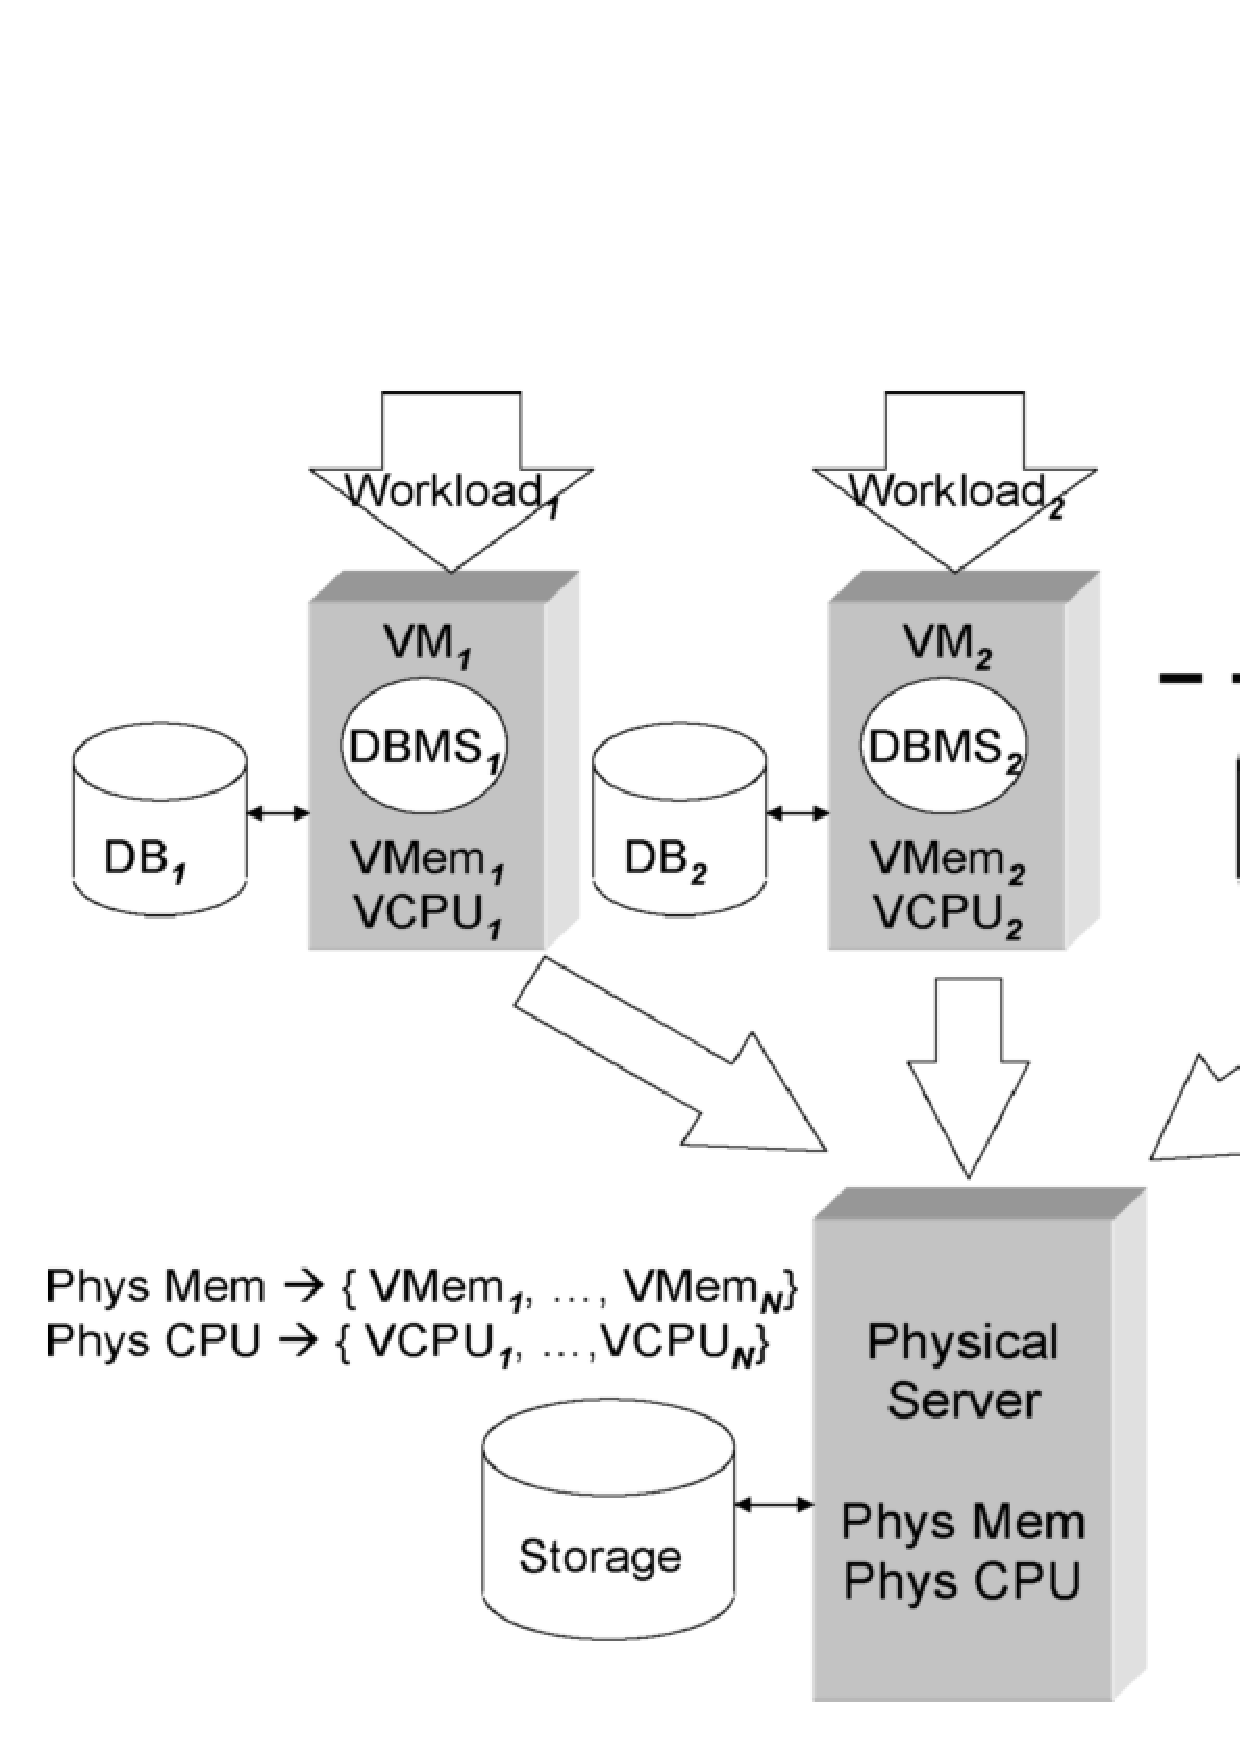
\includegraphics[width=0.8\textwidth]{dbms_consolidation.png}
\caption{Resource Consolidation scenario}
\label{fig:scenario}
\end{figure} 

\section{Problem definition}

In order to model this problem, the author assumes that there are  $M$ types of resources , such as CPU capacity, memory, or I/O bandwidth. The notation used to represent the share of resources allocated to a VM running a workload $W_{i}$ is $R_{i} = [r_{i1},...r_{iM}], 0 \leq r_{ij} \leq 1$. Each workload has the same monitoring interval for all the VMs ( i.e. the workloads represent the statements processed by different DBMSes in the same amount of time ).

Each workload is associated to a cost, which depends on the resource share allocated to the VM in which it runs. The notation $Cost(W_{i},R_{i})$ is used to represent the cost of running the workload $W_{i}$ under resource allocation $R_{i}$. Considering that there are $N$ workloads, the goal is to choose $r_{ij}, 1 \leq i \leq N, 1 \leq j \leq M$ such that 
\[
  \sum_{i=1}^{N} Cost(W_{i},R_{i})
\]
is minimized.

This problem was generalized to satisfy Quality of Service (QoS) requirements. One of these requirements is the possibility to specify the maximum increase in cost that is allowed for a workload under the recommended resource allocation. In order to model this requirement, it was defined a \textit{cost degradation} as
\[
 Degradation(W_{i},R_{i}) = \frac{Cost(W_{i},R_{i})}{Cost(W_{i},[1,...,1])}
\]
, where $[1,...,1]$ represents the resource allocation in which all of the available resources are allocated to $W_{i}$. It can be specified a \textit{degradation limit} $L_{i} ( L_{i} \geq 1 )$, such that 
\[
 Degradation(W_{i}, R_{i}) \leq L_{i}
\]
for all $i$. This limit is set per workload, so it does not need information about other workloads that it will be sharing the physical server with.

Other QoS requirement introduced involves the ability to specify relative priorities among the different workloads. A \textit{benefit gain factor} $G_{i} (G_{i} \geq 1)$ can be used to indicate how important is to improve the performance of $W_{i}$. Each unit of improvement is considered to worth $G_{i}$ cost units. When this parameter is applied to the problem, it may cause a workload to get more resources than its fair share. In order to incorporate it to our problem, the cost equation is modified to minimize the following
\[
  \sum_{i=1}^{N} G_{i} * Cost(W_{i},R_{i})
\]


\section{Architecture}

The process of  determining the allocation of resources to each VM is neither immediate, nor static. The proposed advisor follows a sequence of steps. Initially, it makes a resource allocation based on the workload descriptions and performance goals, which is performed offline ( i.e. the VMs are not running yet ). Then all of the subsequent steps are performed online. It adjusts its recommendations based on the difference between expected and actual workload costs to correct for any cost estimation errors made during the initial phase. At the same time, it uses continuing monitoring information to dynamically detect changes in the workloads. This last step is important because a workload cannot be considered static, its resource needs may change during execution. In both of these online steps, the resource allocation step may occasionally be performed again with updated cost models. This approach prevents the advisor from allocating resources to DBMS instances that will obtain little benefit from them. These resources need to be given to the workloads that need them the most.

Since the advisor does not consist in one single task, it makes sense to organize the flow of its tasks. An overview of this advisor in a modular way is given in ~\ref{fig:architecture}. This paper intends to give a brief explanation of each task.


\begin{figure}[ht]
\centering
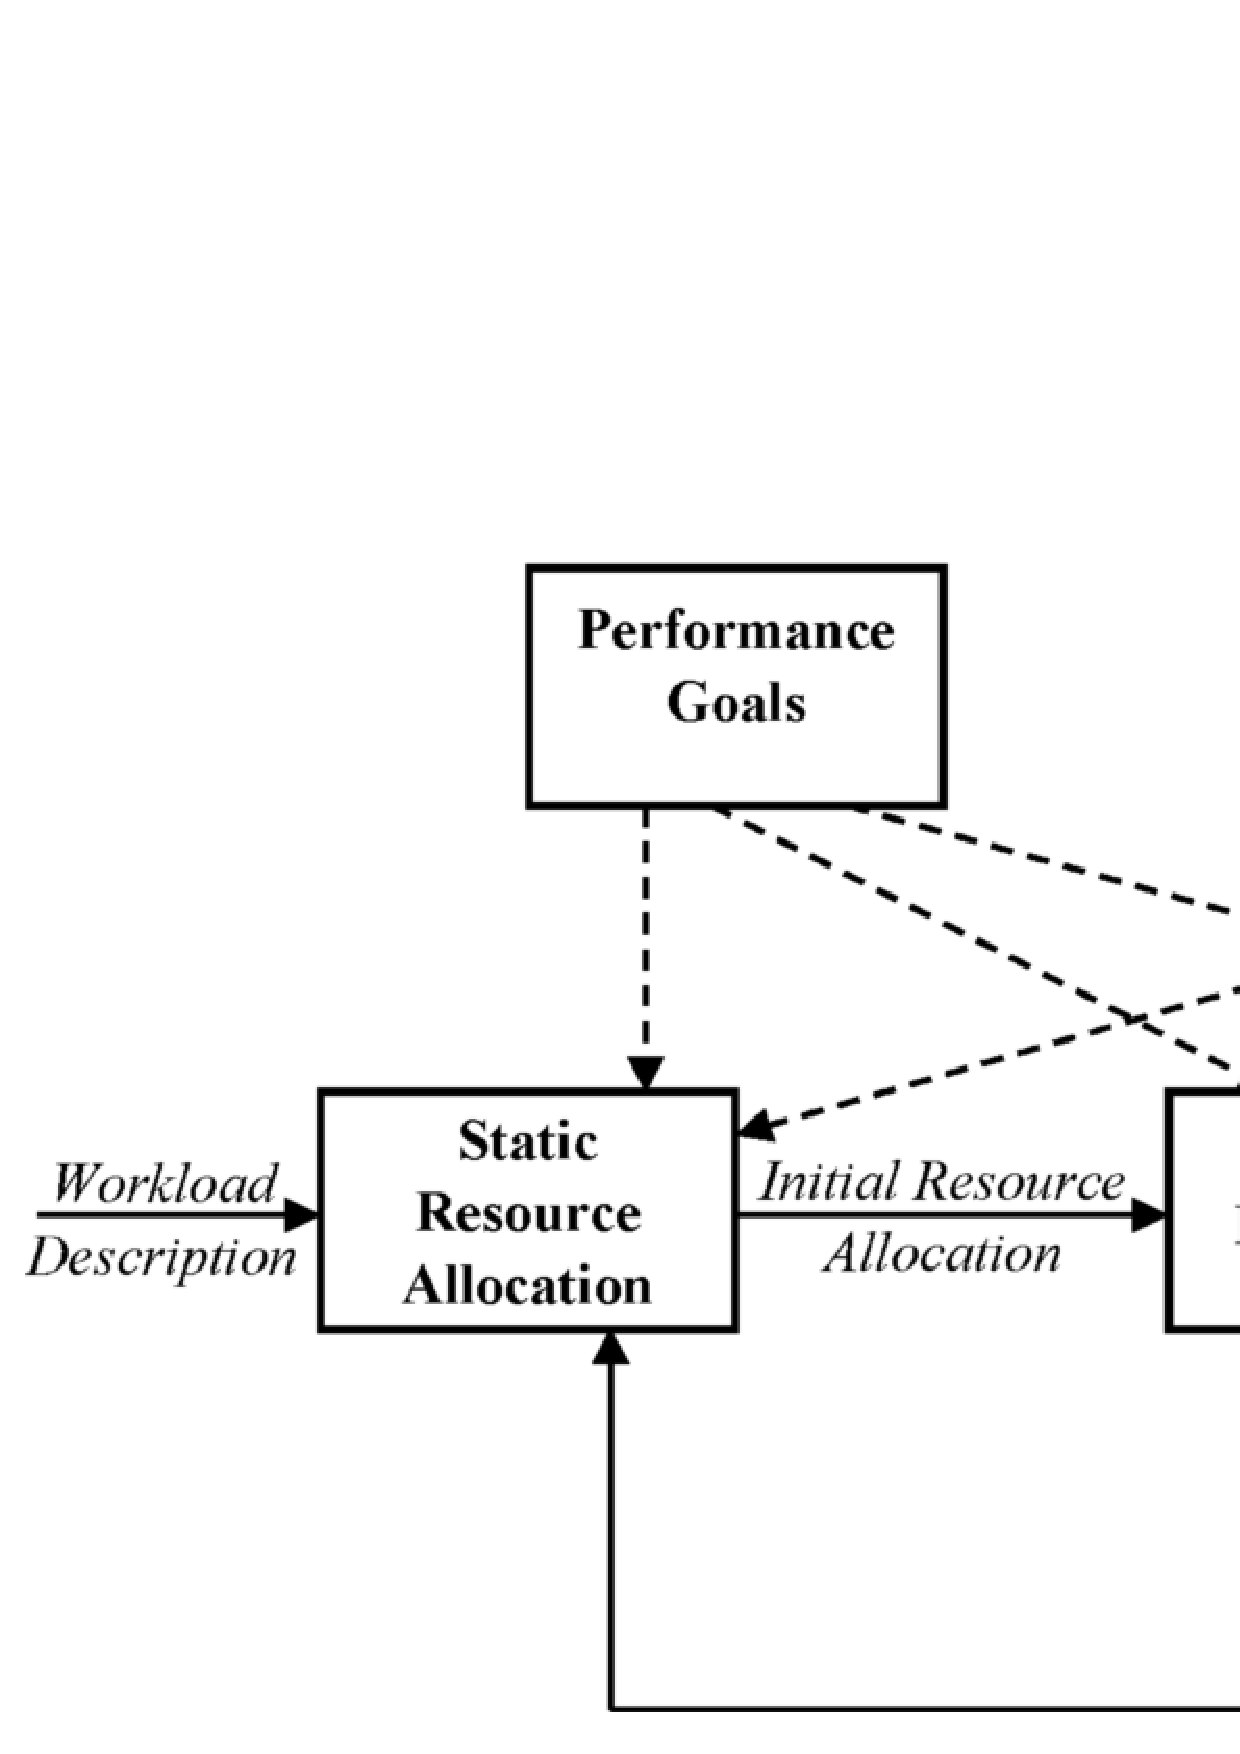
\includegraphics[width=0.8\textwidth]{architecture.png}
\caption{Advisor overview}
\label{fig:architecture}
\end{figure} 

\subsection{Cost estimation and initial allocation}

Given a workload $W_{i}$, the cost estimator will estimate $Cost(W_{i},R_{i})$. The strategy used to implement this module is to leverage the cost models built into database systems for query optimization. The query optimizer cost model can be described as $Cost_{DB}(W_{i},P_{i},D_{i})$, where $W_{i}$ is a SQL workload, $P_{i} = [p_{i1},..,p_{iL}]$ is a vector of parameters that are used to list both the available computing resources and DBMS configuration parameters relevant to the cost model, and $D_{i}$ is  the database instance. 

The author identifies two problems in using only query optimizer cost models. The first problem is the difficulty of comparing cost estimates produced by different DMBSes. They may have different cost models. Even if they share the same notion of cost, the normalization process may differ. This problem is addressed partially by the advisor. It assumes that the DBMSes have the same notion of cost, and it proposes a renormalization step to make $Cost_{DB}(W_{i},P_{i},D_{i})$ from different DBMSes comparable. This step is not considered for implementation, since the support of multiple DBMSes is out of the scope of this paper.

The second problem is that the query optimizer cost estimates depends on $P_{i}$, while the virtualization design advisor is given a candidate resource allocation $R_{i}$. The mapping of these two parameters is achieved through a calibration step. This step determines a set of DBMS cost model configuration parameters according to the different possible candidate resource allocations. It is supposed to be performed per DMBS on the physical machine before running the virtualization design advisor. Once the appropriate configuration parameters $P_{i}$ are determined for every possible $R_{i}$, the DBMS cost model is used to generate $Cost_{DB}$.

The calibration step is performed on  \textit{descritive parameters}, which are used to characterize the execution environment. The approach to the \textit{prescritive parameters}, which control the configuration of the DBMS itself, is to leave it for user definition. For instance, in ~\ref{table:descritive} it is shown some descritive parameters used in PostgreSQL, while in ~\ref{table:prescritive} it is shown the prescritive ones. 


\begin{table}[ht]
    \centering
    \begin{tabular}{ | l | p{5cm} |}
    \hline
    Parameter & Description  \\ \hline
    \textbf{random\_page\_cost} & Cost of non-sequential page I/O \\ \hline
    \textbf{cpu\_tuple\_cost} & CPU cost of processing one tuple \\ \hline
    \textbf{effective\_page\_size} & size of file system's page size  \\
    \hline
    \end{tabular}
    \caption{Descritive parameters}
    \label{table:descritive}
\end{table}


\begin{table}[ht]
    \centering
    \begin{tabular}{ | l | p{5cm} |}
    \hline
      Parameter & Description  \\ \hline
    \textbf{shared\_buffers} & shared bufferpool size \\ \hline
    \textbf{work\_mem} & amount of memory used by each sort and hashing operator. \\
    \hline
    \end{tabular}
    \caption{Prescritive parameters}
    \label{table:prescritive}
\end{table}

The calibration step follows a basic methodology for each parameter $p_{ij} \in P_{i}$, described below:

\begin{itemize}
 \item (1) Define a calibration query $Q$ and a calibration database $D$, such that $Cost_{DB}(Q,P_{i},D)$ is independent for all descritive parameters in $P_{i}$, except for $p_{ij}$; \\
  \item (2) Choose a resource allocation $R_{i}$, instantiate $D$, and run $Q$ under that resource allocation, and measure the execution time $T_{Q}$; \\
  \item (3) This step refers to the renormalization of the $Cost_{DB}$ provided by the DBMS. As mentioned earlier in this section, we are not going into the details of this step; \\
  \item (4) Repeat the two preceding steps for a variety of $R_{i}$ allocations. $r_{ij} \in R_{i}$ only needs to be varied if $p_{ij}$ describes that resource. For instance, query optimizer parameters that describe CPU, I/O and memory are independent of each other and can be calibrated independently. This shall avoid unnecessary calculations; \\
  \item (5) Perform regression analysis on the set of $(R_{i},p_{ij})$ value pairs to determine a calibration function $Cal_{ij}$ that maps resource allocations to $p_{ij}$ values. \\
\end{itemize}

During the described methodology, calibration queries should be carefully chosen. They need to be dependent only on the parameter that is being calibrated. If it is not possible to isolate one parameter, a system of $k$ equations is solved to determine the values for the $k$ parameters.

After the calibration is performed, the advisor is ready to be run. First, it needs to provide an initial configuration. In \cite{Soror:2008:AVM:1376616.1376711}, it was proposed a greedy algorithm to search for an initial configuration, as seen in ~\ref{alg:greedy}.

\begin{algorithm}[H]
 \begin{algorithmic}
    \FOR{$i = 1 \to N$} 
	\STATE $R_{i} \gets [\frac{1}{N},..,\frac{1}{N}]$
    \ENDFOR

   \STATE $done \gets \FALSE$
   \REPEAT
	\STATE $MaxDiff \gets 0$
	\FOR{$j = 1 \to M$} 
	    \STATE $MaxGain_{j} \gets 0$
	    \STATE $MaxLoss_{j} \gets \infty$
	    \FOR{$i = 1 \to N$}
		 \STATE $C' \gets G_{i} * Cost(W_{i},[r_{i1},  r_{ij} + \delta, r_{iM}])$ \COMMENT{Maximize gain}
		 \IF{ $C_{i} - C' > MaxGain_{j}$}
		     \STATE $MaxGain_{j} \gets C_{i} - C'$
		     \STATE $i_{gain} \gets i$
		 \ENDIF
		 \STATE $C' \gets G_{i} * Cost(W_{i},[r_{i1},  r_{ij} - \delta, r_{iM}])$ \COMMENT{Minimize loss}
		 \IF{ $( C' - C_{i} < MaxLoss_{j}) \wedge ( C' satisfies L_{i})$}
		     \STATE $MaxLoss_{j} \gets C' - C_{i}$
		     \STATE $i_{loss} \gets i$
		 \ENDIF
	    \ENDFOR
	    \STATE \COMMENT{Maximum benefit from adjusting this resource}
	    \IF{ $(i_{gain} \ne i_{lose}) \wedge ( MaxGain_{j} - MinLoss_{j} > MaxDiff)$ }
		\STATE $MaxDiff \gets MaxGain_{j} - MinLoss_{j}$
		\STATE $i_{maxgain} \gets i_{gain}$
		\STATE $i_{maxloss} \gets i_{loss}$
		\STATE $j_{max} \gets j$
	    \ENDIF
	\ENDFOR
	\IF{$MaxDiff > 0$}
	    \STATE $r_{i_{maxgain}j_{max}} \gets r_{i_{gain}j_{max}} + \delta $
	    \STATE $r_{i_{maxloss}j_{max}} \gets r_{i_{loss}j_{max}} - \delta $
	\ELSE
	    \STATE $done \gets \TRUE$
	\ENDIF
   \UNTIL{done}

 \end{algorithmic}
  \caption{Greedy search algorithm}
  \label{alg:greedy}
\end{algorithm}
The greedy search algorithm presented initially assigns $\frac{1}{N}$ share of each resource to each one of the $N$ workloads. Then it iteratively considers shifting an amount $\delta$ of resources (e.g. $\delta = 5\%$) from one workload to another. It analyses which workload benefits more from gaining that resource and also which loses less. Based on this, it tries to obtain the maximum benefit from adjusting this resource, and it repeats it for every resource. These adjusts are performed until no more optimizations are possible, condition limited by the \textit{REPEAT} loop . It's also important to notice that this algorithm takes into consideration the QoS parameters discussed earlier in this paper, $L_{i}$ and $G_{i}$.

From results of experiments, the creator of this algorithm observed that the greedy search is very often optimal and always within $5\%$ of the optimal allocation. This result is a good indicative for the algorithm, as it tells us that it hardly gets stuck in local minimums.



\subsection{Online refinement}

The initial allocation is based on the calibrated query optimizer cost model, as described earlier. This enables the advisor to make recommendations based on an informed cost model. However, this model may have inaccuracies that lead to sub-optimal recommendations. The  \textit{online refinement} is based on the observation of the actual times of different workloads running in different VMs. It uses these observations to refine resource allocation recommendations. Then the advisor is rerun with the new cost models, so  we can obtain an improved resource allocation for different workloads. These optimizations are performed until the allocations stabilize (i.e. the new recommendation is equal to the last one ). It's important to notice that the goal of the \textit{online refinement} is not deal with dynamic changes in the workload, which are dealt by another module, but to correct cost models. Thus, it's assumed that the workload is not going to change during this process. 

In order to optimize the recommendations, it is necessary to identify the cost model behaviour. The author identifies two types of models. The first is the \textit{linear model}, which can describe, among other resources, the allocation of CPU. For this resource, workload completion times are linear in the inverse of the resource allocation level. Therefore, the cost model in this case can be represented by
\[
 Cost(W_{i}, [r_{i}]) = \frac{\alpha_{i}}{r_{i}} +\beta_{i}.
\]

The values $\alpha_{i}$ and $\beta_{i}$ are obtained through a linear regression. This regression is performed on multiple points represented by estimated costs for different $r_{i}$ values used during the initial allocation phase. This cost is adjusted by two parameters, $Est_{i}$ and $Act_{i}$, they represent the estimated cost of workload and the runtime cost, respectively. When the cost is underestimated, these parameters are used to increase the slope of our cost equation. From another standpoint, when this value is overestimated, we need to decrease the slope. This is achieved by
\[
  Cost(W_{i}, [r_{i}]) = \frac{Act_{i}}{Est_{i}} * \frac{\alpha_{i}}{r_{i}} + \frac{Act_{i}}{Est_{i}} * \beta_{i}.
\]

However, not all resources are linear. The second type of cost model identified is the \textit{piecewise-linear}, which describes, among others, the allocation of memory. Increasing this resource does not consistently result in performance gain. The magnitude and the rate of improvement change according to the query execution plan. The cost equation is similar to the linear cost model, and it is given by
\[
  Cost(W_{i}, [r_{i}]) = \frac{Act_{i}}{Est_{i}} * \frac{\alpha_{ij}}{r_{i}} + \frac{Act_{i}}{Est_{i}} * \beta_{ij}, r_{i} \in A_{ij}.
\]
The difference here is the parameter $A_{ij}$, which represents the interval of resource allocation levels corresponding to a particular query execution plan, represented by $j$. Its intervals are obtained during the initial phase, when the query optimizer is called with different resource allocations and returns different query execution plans with their respective costs. These query execution plans define the boundaries of the $A_{ij}$ intervals. The end of this interval is the largest resource allocation level for which the query optimizer produced this plan. The initial values of $\alpha_{ij}$ and $\beta_{ij}$ are obtained through linear regression. Together with $A_{ij}$, they are subsequently adjusted.

Both of the equations presented work within their cost model. Nevertheless, a physical  machine has more than one type of resource. Therefore, the author extends the cost equations to multiple resources. In this extension, it is considered that $M$ resources are recommended, such that $M-1$ resources can be modelled using a linear function, while the resource $M$ is modelled using a piecewise-linear function. The cost of workload $W_{i}$, given a resource allocation $R_{i} = [r_{i1},...,r_{iM}]$ can be given by
\[
  Cost(W_{i}, R_{i}) = \sum_{j=1}^{M} \frac{Act_{i}}{Est_{i}} * \frac{\alpha_{ijk}}{r_{ij}} + \frac{Act_{i}}{Est_{i}} * \beta_{ik}, r_{iM} \in A_{iMk},
\]
in which $k$ represents a certain query execution plan, which defines the boundaries of $A_{iMk}$. 

During refinement, this equation is supposed to be performed iteratively, in order to optimize the parameters $\alpha_{ijk}$ and $\beta_{ijk}$. This iteration is shown below.
\begin{eqnarray*}
 Cost(W_{i}, R_{i}) &=& \sum_{j=1}^{M} \frac{Act_{i}}{Est_{i}} * \frac{\alpha_{ijk}}{r_{ij}} + \frac{Act_{i}}{Est_{i}} * \beta_{ik} = \sum_{j=1}^{M} \frac{\alpha'_{ijk}}{r_{ij}} + \beta'_{ik}, r_{iM} \in A_{iMk} \\
 Cost(W_{i}, R_{i}) &=& \sum_{j=1}^{M} \frac{Act_{i}}{Est_{i}} * \frac{\alpha'_{ijk}}{r_{ij}} + \frac{Act_{i}}{Est_{i}} * \beta'_{ik} = \sum_{j=1}^{M} \frac{\alpha''_{ijk}}{r_{ij}} + \beta''_{ik}, r_{iM} \in A_{iMk} \\
  &\vdots&
\end{eqnarray*}

The author in \cite{Soror:2008:AVM:1376616.1376711} proposes an heuristic that changes the equation in the first iteration. Instead of  considering the interval $A_{iMk}$, the first iteration scales to all the intervals of the cost equation (i.e., for all $k$). This is done because the estimation errors can be partly due to a bias in the query optimizer's view of resource allocation levels. In the second iteration and beyond, this cost will be refined according to the interval $A_{iMk}$, where the resource $r_{iM}$ will be scaled.

These refinement iterations stops when the refinement continues beyond $M$ iterations. In this case the refinement process continues, but through a linear regression model to the observed points. At this point, the query optimizer's estimates are just dropped. This process only finishes when the number of iterations reach an upper bound, placed manually. It is used to guarantee termination.

After refining the cost equations, the advisor is rerun. If the newly obtained resource allocation is the same as the original, the refinement process is stopped. Otherwise, it goes on.

\subsection{Dynamic configuration management}

Even if we have an optimal resource allocation, the workload may change its behaviour during execution. They may occur due to the intensity of the workload (e.g. increased number of clients), or the nature of the workload (e.g. new set of queries with different resource needs ). These changes are not dealt by our online refinement, that's why the dynamic configuration management is needed. 

The proposed approach consists in monitoring the relative changes in the average cost per query between periods. If the change in the estimated is above a threshold, $\theta$, we classify this a major change. When this is identified, it's decided to make the virtualization design advisor to restart its cost modelling from initial state, before online refinement. The cost model needs to be discarded, since it no longer reflects information about the workload.

In order to deal with minor changes, it's introduced a new metric $E_{ip}$. It represents the relative error between the estimated and the observed cost of running workload $W_{i}$ in monitoring period $p$. We analyse two consecutive periods. If both $E_{i(p-1)}$ and $E_{ip}$ are below some threshold ( e.g. $5\%$ ), or if $E_{ip} - E_{i(p-1)} > 0$, then we continue with online refinement. In this case, the errors are either small, or are decreasing. Both of these situations can be efficiently dealt by some iterations of online refinement. However, if this condition is not satisfied, the cost model is discarded once again. 
\chapter{\textbf{Cloud infrastructure management}}


This section will be used to described OpenNebula, that is a virtual infrastructure (VI) manager. Organizations can use it to manage and deploy VMs, individually or in groups that must be co-scheduled on local or external resources, which means that it supports hybrid clouds. Some of its key features are:
\begin{itemize}
 \item It provides a homogeneous view of resources, regardless of the underlying hypervisor (e.g. KVM, Xen). This makes the virtualization much less restrictive. The physical machine in which the VM is being run does not need to be tied to a specific virtualization technology, causing incompatibility issues;
  \item Manage a VM's full life cycle, like managing storage requirements and setting up the network;
  \item Supports configurable resource allocation policy.
\end{itemize}

The OpenNebula architecture is illustrated by ~\ref{fig:open_arch}. Each component is specialized in one aspect of VI management. The core takes care of the VM's life cycle. It has three management areas. The first is the preparation of disk images for VMs. It needs to control the image and storage technologies. The second is the network envrironment for them. And finally, it needs to control the hypervisors for creating or controlling VMs. All of these activities are performed through pluggable drivers. This modularity makes the system easier to extend.  


\begin{figure}[ht]
  \centering
 \includegraphics[scale=0.4]{opennebula_arch.png}
  \caption{OpenNebula architecture}
  \label{fig:open_arch}
\end{figure}



% However, the scope of this paper is limited to the private part of the cloud, since it's neither possible, nor makes sense to balance the load of an external provider infrastructure.






\chapter{\textbf{Implementation}}

\label{chap:implementation}

In this chapter, it's discussed the virtualization design advisor implementation over OpenNebula. Our aim is to optimize the distribution of resources inside a private cloud for VM guests running database workloads. However, in order to make this work feasible, some restrictions were made. The major restriction involves the list of resources which would be modelled and optimized. In this paper, this was limited to CPU. Further restrictions were established, and they'll be explained as the advisor is detailed.

For organizational purposes and better integration with OpenNebula, our solution  is part of a module called OpenRC, which stands for Open Resource Consolidation. It was designed to work alongside OCA, since it will need full access to OpenNebula functionality. As OCA, it was also implemented in Ruby\footnote{http://www.ruby-lang.org} language. In this module, it was implemented both the steps presented in figure ~\ref{fig:architecture}, from chapter ~\ref{chap:virtualization}, and missing features from OpenNebula, needed for the advisor.

One of the missing features in OpenNebula is the ability to dynamically reallocate resources,as mentioned in chapter ~\ref{chap:infrastructure}. Although it is not supported by OpenNebula, most hypervisors currently support it for some types of resource. Besides the need for changes in the OpenNebula drivers to support these operations, it would be necessary to extend the OpenNebula's core to handle them. Instead, it was decided to implement this functionality in OpenRC, with information provided by OCA. The approach to achieve this  was the use of libvirt\footnote{http://libvirt.org/}, which defines itself as "A toolkit to interact with the virtualization capabilities of recent versions of Linux (and other OSes)". It offers an API that works with all the hypervisors supported by OpenNebula, offering many features, including CPU limitation. Currently, OpenNebula already has a libvirt API, which enables VM management over the core layer. OpenRC uses libvirt at a lower level, correspondent to OpenNebula's 
bottom layer. At this time, libvirt has three parameters that allows us to control the cpu scheduling. Here is an explanation of their use:
\begin{itemize}
 \item \textbf{quota} and \textbf{period}: These parameters work together, they allow us to set a hard limit for the cpu usage. \textbf{Period} should be in range $[1000, 1000000]$. Within it, each virtual CPU of the VM will not allowed to consume more than \textbf{quota} worth of runtime. For instance, the following values define that the VM guest will be limited to $20\%$ of CPU time:
  \begin{itemize}
   \item  \textbf{period}$=100000$; 
   \item \textbf{quota}$=20000$;
  \end{itemize}
  \item \textbf{shares}: Opposite to the previous parameters, \textbf{shares} enables us to set a soft limit for CPU usage. It specifies the proportional weighted share for the VM guest. Its value is relative. For instance, a VM configured with value $2048$ will get twice as much CPU time as a VM with value $1024$. However, if the CPU is not being used by the VM with a higher parameter value, the other will not be denied CPU idle time.
\end{itemize}

These parameters are indirectly updated and retrieved through a class called \textbf{CPULimitation}, within OpenRC. The objective of this class is to set hard/soft limits for CPU usage of OpenNebula VMs on remote hosts. Our approach to execute these remote commands  is the same as OpenNebula, in fact for this task we only import the OpenNebula's class \textbf{RemotesCommand}, which is responsible for executing OpenNebula commands through SSH\footnote{Secure Shell} on remote hosts.

Other implemented feature was the communication with the DBMS running inside the VM guest. This was achieved by the creation of the \textbf{DatabaseHelper} class. Structured according to the facade pattern, it enables access to a set of classes, responsible for establishing a database connection, set tuning parameters, process single queries or workloads, obtain estimated and actual runtime costs, etc. This pattern was chosen to make the support of other DBMSes easier in future work. For the purposes of this paper, only PostgreSQL\footnote{http://www.postgresql.org/} was supported and tested as DBMS. This decision was not only based on implementation details, but also to ease cost modelling and parameter calibration. The support of a new DBMS starts by the creation of a module, representing the DBMS. In this module,  it should be defined classes which have its functionality exposed by \textbf{DatabaseHelper}, as illustrated by figure ~\ref{fig:facade}. As these classes have database specific methods, 
they shouldn't be 
directly implemented in the facade object. For instance, when a query is run for analysing purposes, the costs are not obtained the same way for different DBMS types. Once the database module is created, following specific implementation rules, it can be easily included. 

\begin{figure}[ht]
  \centering
 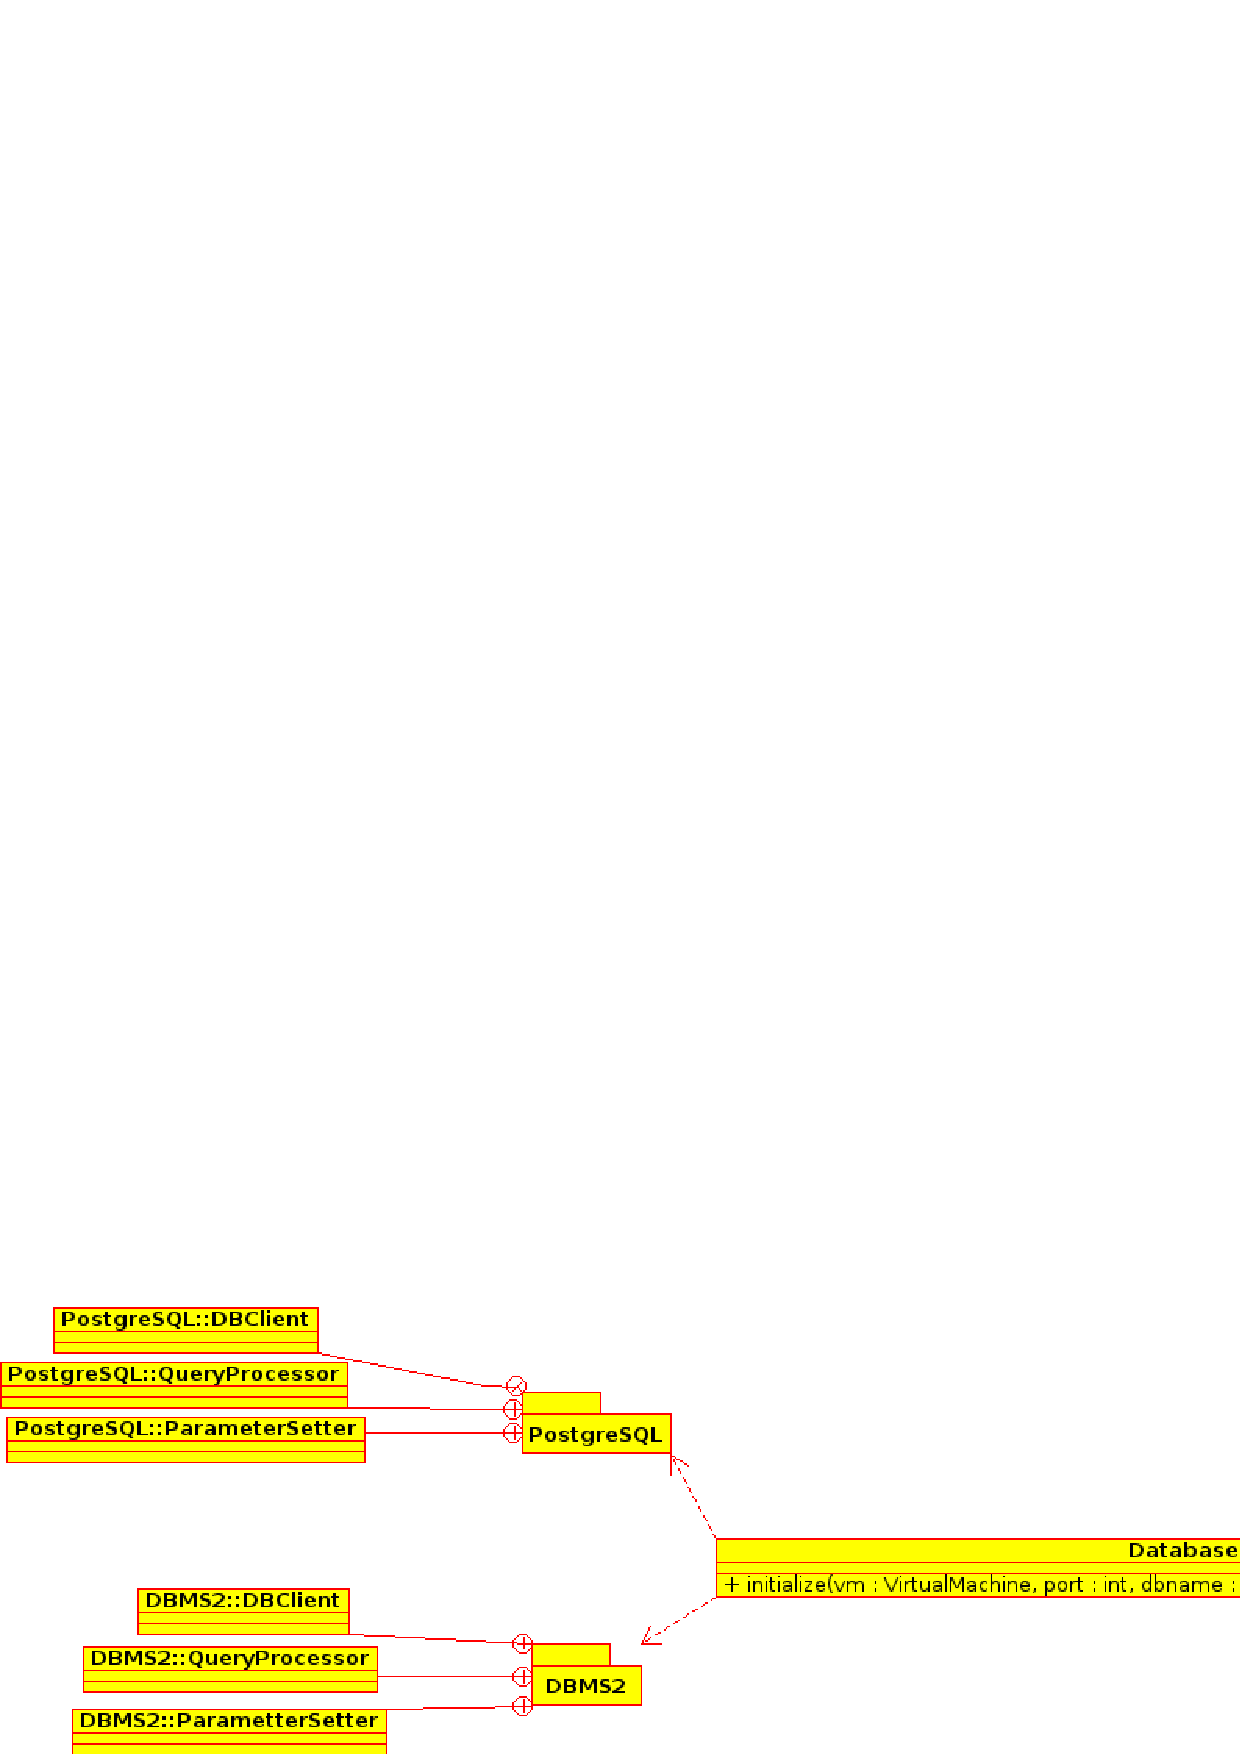
\includegraphics[scale=0.5]{database_helper_facade.png}
  \caption{DatabaseHelper facade with an eventual support of a second DBMS}
  \label{fig:facade}
\end{figure}

A \textbf{DatabaseHelper} instance needs to be initialized with a \textbf{VirtualMachine} object, defined in OCA. As mentioned in chapter ~\ref{chap:infrastructure}, OpenNebula is able to define both the MAC and IP address of a Virtual Machine, in form of a lease. It also keeps track of these leases in its SQL Pool. As any other pool element, this information can be retrieved through OCA, in XML format. So when a VM is passed to our class, it's possible to retrieve the IP address of that VM and connect to PostgreSQL. As some authentication parameters ( database name, user name, user password ) are also needed for database connection, and they are not stored by OpenNebula SQL pool, they must be passed manually to our solution.

As soon as the communication with the DBMS and the CPU limitation were implemented, it was possible to start developing modules inherent to our advisor. In the following subsections, every part of the process has its implementation detailed.

\section{Calibration}
\label{sec:calib}

The first step in order to implement the advisor is the creation of a calibration process. As discussed earlier, this task is responsible for mapping the query optimizer's cost model, which depends on its parameters $P_{i}$, to  the advisor's cost model, based on resources $R_{i}$. Without it, it's not possible to build a proper cost estimator. Since the calibration should be performed before any VM deployment on each physical host on our cloud, it was decided that this process should become an OpenNebula hook. The hook definiton is given below:
\begin{itemize}
 \item HOST\_HOOK $=$ [ \\
    name      $=$ "Calibration",\\
    on        $=$ "CREATE",\\
    command   $=$ "openrc/host\_db\_calibration.rb",\\
    arguments $=$ "\$HID",\\
    remote    $=$ no ]\\
\end{itemize}

This hook will execute the host\_db\_calibration.rb script on the OpenNebula server whenever a new host is created, passing the host id as argument. In this script, the whole calibration process is performed, as described in chapter ~\ref{chap:virtualization}. Initially, it searches for the image of a specific VM, which basically contains the calibration database. As hosts and virtual machines, images are also objects managed by OpenNebula. Thus, it needs to be added to the image pool before running the calibration script.

The calibration database running inside the VM is generated by pgbench\footnote{http://www.postgresql.org/docs/devel/static/pgbench.html}. This tool is able to run benchmark tests, based on TPC-B, for PostgreSQL. During implementation, it was only used to generate and populate our calibration database. Its choice relies on its integration with PostgreSQL, usability, and the ability to populate databases with custom sizes.

Once the calibration database is up and running, it's necessary to run specially designed queries to find out the relation between different resource allocation levels and tuning parameters costs.  As mentioned in subsection ~\ref{subsec:cost}, DBMSes don't generally share the same notion of cost. It means that we also must find the relation between DBMS estimated costs and actual costs, which would be the execution times. In PostgreSQL, all costs are normalized with the respect of time required for a single page to be fetched from disk. This cost is represented by the parameter $seq\_page\_cost$. Therefore, by finding it's actual value, we also find this relation. 


Our approach to find the actual cost values for $seq\_page\_cost$ was to use a tool to find the virtual disk throughput. In this implementation, the tool hdparm\footnote{http://sourceforge.net/projects/hdparm/} was chosen. Among other features, this utility serves as a disk benchmarking alternative for Linux. It must be previously installed in the calibration VM. Its results are obtained through a specially designed PostgreSQL function, added to the calibration database. Based on the results retrieved from this function, the cost of $seq\_page\_cost$ is calculated. Besides this calculation, it's also important to decide how to simulate I/O disk contention at this step. This would happen in production environments, where multiples VM guests are run concurrently. Calculating $seq\_page\_cost$ without considering a realistic scenario could lead to inaccurate results. It was decided to magnify this problem by stressing the host disk while the costs are being generated and retrieved. The stress\footnote{
http://freecode.com/projects/stress} utility was chosen to generate disk stress. It's used to spin several 
workers writing on files and removing directory entries on the remote host. In a more realistic setup, the VMs would compete less for I/0, and probably this cost would have a certain variability. By stressing the disk, our aim is to simulate a worst-case scenario. 


After finding the relation between the DBMS estimated cost and the actual cost ( execution time ), it's possible to calibrate the tuning parameters. Since this paper is restricted to reallocate CPU among VMs, only parameters that describe CPU need to be calibrated. For PostgreSQL, these are shown below.

\begin{table}[ht]
    \centering
    \begin{tabular}{ | l | p{5cm} |}
    \hline
    Parameter & Description  \\ \hline
    \textbf{cpu\_operator\_cost} & Cost of processing each operator or function call \\ \hline
    \textbf{cpu\_tuple\_cost} & Cost of processing one tuple (row) \\ \hline
    \textbf{cpu\_index\_tuple\_cost} & Cost of processing each index entry during an index scan  \\
    \hline
    \end{tabular}
    \caption{Parameters that describe CPU}
    \label{table:descriptive}
\end{table}


PostgreSQL uses these parameters to build its query optimizer's cost estimates. That's why a lot of documentation can be found on how to tune these parameters in order to obtain better cost execution plans. However, the way these parameters are exactly used within these plans is poorly documented. Only by observing the source code is possible to determine how they are applied to simple query plans. The first two parameters at table ~\ref{table:descriptive}, $cpu\_tuple\_cost$ and $cpu\_operator\_cost$ can be obtained by the query presented at subsection ~\ref{app:cal1}. Without changing the values of any PostgreSQL's default parameter values, this query will always have the same execution plan generated. It will access the table $pgbench\_accounts$ using a sequential scan, and subsequently perform an aggregation. PostgreSQL has the following equations for these two operations:
\begin{equation}
  \begin{split}
      SEQSCAN &= ( seq\_page\_cost * num\; pages \; fetched ) + ( cpu\_tuple\_cost * number\; rows ) \\
      AGGREGATE &= SEQSCAN + ( cpu\_operator\_cost * number\; rows) \\
  \end{split}
\end{equation}

The estimated cost and execution times for these equations can be obtained by executing this query on PostgreSQL with the command $EXPLAIN (ANALYZE)$. In this case, the query will be actually executed and an execution plan will be returned. Each step in the execution plan has its corresponding costs indicated. This means that it's possible to isolate costs for each operation from the total. Based on the actual costs returned, our script is able to deduct the parameters from the equations. However, by retrieving these costs we get a different scale, as the actual costs are in milliseconds, instead of page fetches. We use the actual value of $seq\_page\_cost$ to make conversions between different scales. The equation is given below:
\[
 param_{estimated} = \frac{param_{actual}}{seq\_page\_cost_{actual}}
\]

To calculate the first two descriptive parameters, only one modification to the original equation was made. PostgreSQL considers the cost fetching pages  during a $SEQSCAN$. The problem is to determine how many pages were actually fetched from disk. One approach would be running the query with the command $EXPLAIN (ANALYZE,BUFFERS)$. By using this command, it's informed the number of pages hit in the PostgreSQL cache and number of pages that needed to be read. However, the PostgreSQL cache may not reflect the state of the operating system cache. During experimentations, changes in the hit/miss ratio did not incur in an expected change in actual costs. Our approach was to cache all the data for the consults and limit the number of page accesses of a determined query. After doing that, costs related to disk page fetches were ignored from the equation.

The third descriptive parameter, $cpu\_index\_tuple\_cost$ , is used during index scans. It can be obtained through the query presented in subsection ~\ref{app:cal1}. Before running this query, it is necessary to set the following parameter:
\[
 enable\_seqscan=off
\].
This will force the planner to use an index scan plan, as $aid$ is a primary key, instead of a sequential scan. Its equation is much more complex than the previous one. Mainly because it involves a lot of I/O cost estimates. In addition to $seq\_page\_cost$, its plan is highly dependable on another parameter, namely $random\_page\_cost$. It represents the cost of fetching a non-sequentially disk page. During estimation, PostgreSQL uses an approximation of pages actually fetched after accounting for cache effects. This approximation is proposed in \cite{Mackert:1989:ISU:68012.68016}. The number of fetched pages is

\begin{eqnarray*}
  PF=&& \\
  &min(2TNs/(2T+Ns),T)\qquad \qquad \qquad & when\quad T \le b \\
  &2TNs/(2T+Ns) & when \quad (T > b) \wedge (Ns \le 2Tb/(2T-b)) \\
  &b + (Ns -2Tb/(2T-b))*(T-b)/T & when \quad (T > b) \wedge (Ns > 2Tb/(2T-b)) \\
\end{eqnarray*}
where
\begin{description}
 \item T $=$ number of pages in table;
 \item N $=$ number of tuples in table;
 \item s $=$ selectivity $=$ fraction of table to be scanned;
 \item b $=$ number of buffer pages available.
\end{description}

For the same reasons why I/O cost was discarded for the first equation, we decided to eliminate it from the $cpu\_index\_tuple\_cost$ calculation. Since we are only interested in CPU cost, instead of I/0, we cache all the data to be retrieved and consider the following parameters to be
\begin{equation}
 \begin{split}
  seq\_page\_cost &= 0 \\
  random\_page\_cost &= 0
 \end{split}
\end{equation}

Given this configuration, the equation for a single index scan can be defined as
\begin{eqnarray*}
  \lefteqn{Cost=} \\
  &&ntuples * ( cpu\_index\_tuple\_cost + qual\_op ) + \\
  &&100*cpu\_operator\_cost + \\
  &&cpu\_per\_tuple\_cost * ntuples + ( I/0\;Cost ) \\
  \lefteqn{qual\_op=} \\
  &&cpu\_operator\_cost * ncond \\
  \lefteqn{cpu\_per\_tuple\_cost=} \\
  &&cpu\_tuple\_cost + cpu\_operator\_cost * nfilters
\end{eqnarray*}
,where
\begin{description}
 \item ntuples $=$ number of tuples retrieved;
 \item ncond $=$ number of index conditions;
 \item nfilters $=$ number of filters ( including index conditions );
 \item I/O cost $=$ indicates the cost of fetching pages from disk, related to parameters $seq\_page\_cost$ and $random\_page\_cost$. As it is discarded by the calibration process, it won't be detailed.
\end{description}

The values for $cpu\_tuple\_cost$ and $cpu\_operator\_cost$, the details about our calibration query and database are already known. As we discared the I/O cost from our equation, there is only one variable left to be deducted, that is $cpu\_index\_tuple\_cost$. The calibration process then isolates this variable from the rest of the equation and finds its value under different resource allocations, like it was done for the two first parameters. The library built to enable CPU limitation is used here to set a hard limit for CPU usage.

The execution costs found during the calibration step are then stored in files, with the corresponding CPU allocation levels. The collected data is used later by the virtualization design advisor. 

\section{Virtualization Design Advisor}

After the end of the calibration process for a certain host, the virtualization design advisor can start handling database workloads and resource allocation levels. The advisor modules, shown in figure ~\ref{fig:architecture}, served as a base on how to organize our implementation. This can be seen on figure ~\ref{fig:advisor}. Here, a new process was added, namely \textbf{LoadGenerator}.  Its task is to run the workloads under resource allocations conditions established during \textbf{GreedySearch}. The costs obtained through execution are passed to both \textbf{OnlineRefinement} and \textbf{DynamicConfigurationManagement}. During workload execution, this class may call \textbf{GreedySearch} several times for reallocation, regarding changes in the workload or recurrent allocation optimizations. In this section, each class within the advisor will be detailed.


\begin{figure}[ht]
\centering
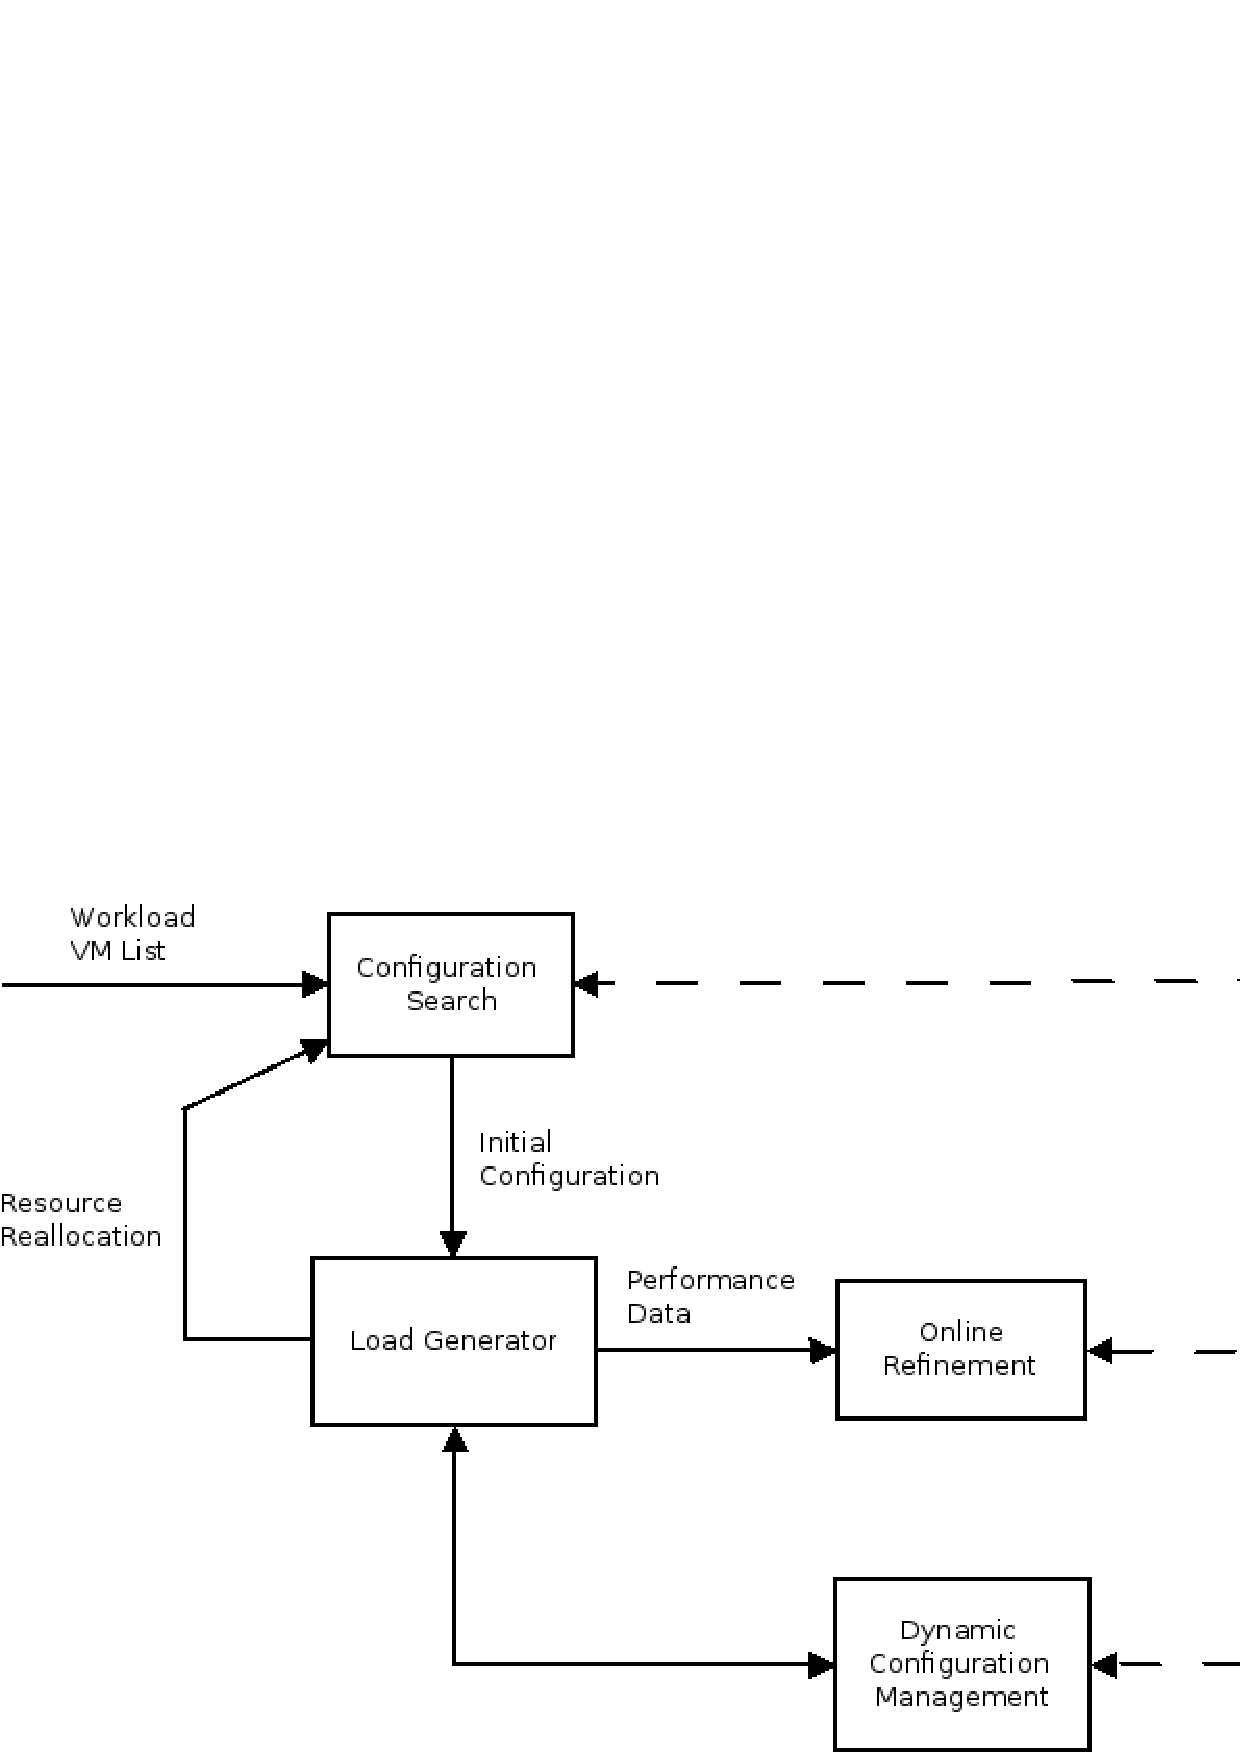
\includegraphics[width=0.8\textwidth]{advisor-arch.png}
\caption{Implementation overview}
\label{fig:advisor}
\end{figure} 

\subsection{Greedy Search}

The \textbf{GreedySearch} class, from which the advisor is started,  is an implementation of the algorithm presented in section ~\ref{sec:greedy}. This is the only class that actually changes the resource allocation levels. Considering that a private cloud is composed of multiple hosts, it is necessary to run multiple instances of this class. It was created a daemon to manage these multiple searches. It waits for virtual machines to be started and also for workloads to be run on these VMs. Then it resends this information to the \textbf{GreedySearch} instance that corresponds to the host in which that particular VM was designated to be run. Information about newly created VMs can be automatically added as soon as they are created, through a OpenNebula hook. On the other hand, workloads are sent with a script, which sends their information through a TCP Socket, in an expected format.

The search is used in three occasions. The first is when the advisor is started. The objective, in this case, is to find a better initial allocation than the default ( i.e. find an allocation of resources for the $N$ VM guests better than the proportion $\frac{1}{N}$ ). It relies on estimates provided by the \textbf{CostEstimator} class to accomplish it. In a production environment, a good approach would be to base these estimates in a workload history. As we only have a testing scenario, it was opted to base our search on the first workload that is yet to be run.

In the other two occasions, the search is called by the \textbf{LoadGenerator} class. The first is related to the online refinement process, described in subsection ~\ref{subsec:ref}. As the cost estimator model is refined after each workload execution, new calls are made to reflect these refinement changes in the resource allocation. In this case, the searches are not restarted from the default allocation, instead we search for improvements to the current allocation. If the allocation remains the same, this search will not be called any longer by \textbf{LoadGenerator}. And finally, the last occasion happens when a workload change is detected. Then \textbf{LoadGenerator} calls this class, and the search will be started from scratch. This case is similar to the first search, as both of them start from the default allocation and the cost model is restarted.

Independently on how the search is called, it always ends by applying the resource allocation levels found. \textbf{GreedySearch} is the only class within the advisor that actually changes them. This is applied in two steps. The first corresponds to setting a soft limit on the CPU level for each VM, according to the resource allocation levels found during search. The second step is to set the parameters for each DBMS, also according to the search. After they are applied, the rest of the workload can be run.

\subsection{Cost Estimator}

The cost estimation process is performed by the class \textbf{CostEstimator}. The description of how this task should be performed in the virtualization design advisor is given in subsection ~\ref{subsec:cost}. Basically, it needs to provide an estimated cost for running a certain workload under a determined resource allocation level. During initial calls to this estimator, the cost model is not built yet. So \textbf{CostEstimator} leaves this task to be performed by the cost estimator built inside the DBMS query optimizer. Here we face a problem described previously, while our cost model depends on a resource allocation $R_{i}$, the query optimizer cost estimates depend on a set of tuning parameters $P_{i}$. This mapping has already been performed in the calibration process. Therefore, this class collects all calibration data for the tuning parameters and uses linear regression on the observed points. 

The equations obtained through linear regression for each parameter will be used to map $R_{i}$ to $P_{i}$. Besides being useful to the \textbf{CostEstimator} class, they also help the \textbf{GreedySearch} class to know how to set the DMBS parameters under a certain resource allocation level. They stop being used for cost estimation purposes when the cost model is built. Our approach to build the cost model is by keeping statistics of previous calls to this class. During an initial search, \textbf{CostEstimator} may be called several times for different resource allocation levels, and so the estimated results are stored. Before running the workload, a linear regression is performed on these points. As in \cite{Soror:2008:AVM:1376616.1376711} CPU is described as a resource that varies linearly, a linear regression model provides a good approximation. After building the cost model, this class stops calling PostgreSQL for estimates. This significantly reduces the extra calls to the DBMS. So the advisor is 
expected to have a better performance as it is being run.

Other difference between our cost estimator and the one built inside the query optimizer is the scale used. Our approach was to use use costs based on query runtime. The reason is that this is easy to determine and a better approach to compare different DBMSes. As already mentioned in section ~\ref{sec:calib}, PostgreSQL has a different notion of cost. Like it was done during the calibration process, we simply use the actual value of $seq\_page\_cost$ to convert between the two scales. Our renormalization equation is
\[
 Cost(W_{i}, [r_{i}]) = Cost_{DB}(W_{i},P_{i},D_{i}) * seq\_page\_cost_{actual}
\]

. Once the cost model is built and the we are able to renormalize the cost, it can be refined by the \textbf{OnlineRefinement} class.

\subsection{Online Refinement}

The online refinement process adopted in our advisor is straightforward. Considering that the CPU has a linear model and that we only need to refine this resource, the \textbf{OnlineRefinement} class  is an implementation of the first refinement equation presented in subsection ~\ref{subsec:ref}. This equation is designed specifically for refining resources with linear variation. During execution, the cost model is refined the following way:
\begin{equation}
 \begin{split}
   Cost(W_{i}, [r_{i}]) & = \frac{\alpha_{i}}{r_{i}} +\beta_{i} \\
   Cost'(W_{i}, [r_{i}]) & = \frac{Act_{i}}{Est_{i}} * \frac{\alpha_{i}}{r_{i}} + \frac{Act_{i}}{Est_{i}} * \beta_{i} = \frac{\alpha_{i}'}{r_{i}} +\beta_{i}' \\
   Cost''(W_{i}, [r_{i}]) & = \frac{Act_{i}}{Est_{i}} * \frac{\alpha_{i}'}{r_{i}} + \frac{Act_{i}}{Est_{i}} * \beta_{i}' = \frac{\alpha_{i}''}{r_{i}} +\beta_{i}'' \\
    & \vdots
 \end{split}
\end{equation}

 . $\alpha_{i}$ and $\beta_{i}$ are parameters of the linear model for workload $W_{i}$, and $Act_{i}$ and $Est_{i}$ are the actual and estimated costs for running this workload, respectively. In order to apply these equations, this class needs to receive the estimated and the actual costs for this workload. The actual runtime costs are provided by the \textbf{LoadGenerator} class, and the estimated costs come from the \textbf{CostEstimator}. The latter will have then its cost model updated through the refinement performed.

\subsection{Load Generator and Dynamic Configuration Management}

The \textbf{LoadGenerator} class was added to the advisor with the objective to simply run the workloads. Besides increasing the cohesion among the advisor classes, it helps us to determine which parts of the advisor we want to enable. Both the online refinement process and the workload change detection may be disabled in order to test a specific scenario in the advisor.

This class launches a thread for each VM running on a certain host, in order to run the workloads concurrently. Each VM is designated a workload queue. Even though workload units may be received from multiple clients, they are stored in a single queue, which is processed sequentially. This definitely differentiates our tests from a production environment, where a database may receive multiple queries concurrently. It limits our advisor in testing workload intensities. Therefore, in this paper our results are focused on the workload nature, rather than its intensity. As the execution results are obtained, they are passed to \textbf{OnlineRefinement}, if it is enabled. 

While the \textbf{LoadGenerator} runs the queries for each workload, the \textbf{DynamicConfigurationManagement} monitors this execution periodically. 
It is a simplified version of the module described in subsection ~\ref{subsec:dcm}. Every monitoring period, it checks for relative changes in the cost per query. If the change is above a threshold $\theta$ ( i.e. it's a major change ), it reports it. Otherwise, the changes are ignored.

The relation between these two classes was implemented according to the observer pattern. \textbf{LoadGenerator} acts as the observer, although it only starts observing the class after all the cost models have been defined. If a major change in the workload is detected by \textbf{DynamicConfigurationManagement}, it notifies the observer . When this happens, the \textbf{LoadGenerator} class decides to restart from the greedy search process, discarding the cost model.

One of the virtualization design advisor  features that was left out in this implementation was the support of QoS parameters. This means that during execution, all the workloads are treated equally, and no retsrictions are made to their improvement or decrease in performance. The implementation of the \textit{benefitial gain factor} and the \textit{cost degradation} will be left for future work.




%In this paper, it's proposed an implementation of the virtualization design advisor over OpenNebula. The aim is to optimize the distribution of resources inside the private part of a cloud for VMs running database workloads. Since it's not possible, nor makes sense to optimize an external provider's infrastructure, the public part of the cloud is just ignored. We also stick to the PostgreSQL\footnote{http://www.postgresql.org/} as the DBMS used in our solution, although the support for other DBMSes could be extended in future work.

%As already described, the virtualization designer advisor has only been modelled and tested against one server. There are two issues in porting this solution to a cloud. First, a cloud can contain several hosts, instead of one. Other issue is that a cloud is a heterogeneous environment. In spite of the homogeneous view of resources provided by the VMM, the hosts may be different themselves. To address these problems, the proposed approach consists in having $N$ instances of our advisor, being $N$ the number of nodes in the private cloud. Therefore, the advisor will not see the cloud as a whole, but only the host it was assigned to work with, the same as it was working with only one server. 

%The first step of this implementation would be the creation of a module responsible for the calibration process. As discussed earlier, this calibration will be used to map the query optimizer's cost model, which depends on its parameters $P_{i}$, to  the advisor's cost model, based on resources $R_{i}$. This process is supposed to be executed before any VM deployment, since the initial allocation depends on the latter cost model. Thus, it will be executed whenever a new physical host is added to a cluster. As this paper is limited to one DBMS, the renormalization step will  not be performed.


%After calibration, we expect the OpenNebula's default scheduler to define which host will be assigned to the VM that is to be deployed, as usual. At this step, the only provision that needs to be taken is to set the \textit{RANK} variable properly. In this paper, we intend to deal with only two types of resources: memory and CPU. Therefore, we propose the following heuristic for the \textit{RANK}:
%\begin{itemize}
% \item \textit{RANK} $=$ $\alpha *$ \textit{FREECPU} + $ (1 -\alpha) *$ \textit{FREEMEMORY}, $  0 \le \alpha \le 1  $.
%\end{itemize}
%In this equation, we expect $\alpha$ to be used to prioritize one type of resource over another. Since the scheduler assigns the host before being possible to run the advisor, this heuristic will be used for all kinds of workloads. So it doesn't matter whether they are more or less CPU intensive or memory intensive. We consider this to be a limitation. However, we still expect that this heuristic will be able to  distribute well the VMs among the hosts.

%Once the VMs are placed on a machine, the initial configuration step from the virtualization design advisor can be started. In order to deal with their initial configuration, it's proposed the use of the greedy search algorithm, described earlier in this paper. A problem that has already been identified, which affects the greedy algorithm, is the lack of current support for dynamic resource reallocation in OpenNebula. One possible approach would be the use of libvirt\footnote{http://libvirt.org/}, which defines itself as "A toolkit to interact with the virtualization capabilities of recent versions of Linux (and other OSes)". It offers an API that works with all the hypervisors supported by OpenNebula, offering many features, including resource reallocation. Currently, OpenNebula has an libvirt API, which enables this tool to manage the VMs over the core layer. It should be possible to implement a solution by using libvirt under the core layer, to extend the drivers' capabilities too.

%The online refinement and the dynamic configuration management steps should have direct implementations, following their descriptions. The initial configuration is defined by the greedy algorithm ( the static resource allocation module ), it stops when it finds the best allocation, which may be the optimal or close to it. Once this task is performed, the online refinement is started. It updates the cost model by observing estimated and actual times of workloads.  It returns an optimized cost model to the first step, where the greedy algorithm is restarted and searches for a new recommendation with the optimized cost model. The optimizer only stops when the newly obtained recommendations don't differ from the original ones (i.e. it stabilizes ). The dynamic configuration management module is also started after the the end of the initial configuration. It also uses optimized cost models to monitor changes in the workload. It may restart the workload when major changes are detected.

%The performance of this advisor is expected to improve as optimized cost models are obtained, and so less calls to the DBMS's query optimizer are needed. This is due to the fact that these calls have a high computational cost.



\chapter{Results}

\label{chap:results}

The experiments were conducted using the PostgreSQL 9.0.7 as the database system. Because of the nature of the advisor, all tests were performed on a single host from a cluster managed by OpenNebula 3.6. The host has one 2.4GHz dual core processor and 4GB RAM, running Fedora Linux 16, using kernel version 3.3.8. Even though the the library created to reallocate CPU in OpenRC should work with all the hypervisors supported by Libvirt, the experiments were only performed with KVM\footnote{http://www.linux-kvm.org/}. This hypervisor is already integrated within the mainline Linux kernel since the 2.6.0 kernel version. It was designed to support only hardware assisted virtualization.

\section{Calibration}

During the calibration step, a special VM was created to be run on newly added hosts. It runs the Debian Squeeze Linux operating system, specially configured to be a database server. It contains a 300MB TPC-B database, created with PGBench. Under the tested host, the VM was given both CPU cores and 2GB of RAM. Considering the database size, the whole database is loaded in memory. This decision does not have any impact, since only the parameters that describe CPU should be calibrated, instead of I/O. The memory storage for PostgreSQL was created using standard features provided by the DBMS and Linux operating system. The PostgreSQL init scripts were modified to automatically handle this storage every time the database service is stopped or started, including the VM booting. As the calibration queries have a simple known query plan, the tuning parameters are only modified if their change has an effect in the query optimizer decisions. Otherwise, their default values are not modified.

The parameters \textbf{cpu\_tuple\_cost} and \textbf{cpu\_operator\_cost} were calibrated using the query shown in subsection ~\ref{app:cal1}. The values obtained for different resource allocations are shown in figures ~\ref{fig:cpuop} and ~\ref{fig:cputp}, along with the linear regression performed on them. Based on these results, it is possible to observe that the parameters that describe CPU do not have a strict linear variation, as seen on  \cite{4401021}. However it contradicts  \cite{Soror:2008:AVM:1376616.1376711}, which affirmed that this variation was linear when the memory for the VM was allocated to $50\%$. Considering the linear equation to be
\[
 f(x) = m*x + b
\],
the asymptotic errors found were the following:
\begin{itemize}
 \item \textbf{cpu\_tuple\_cost}
 \begin{itemize}
  \item $m \approx 6,7\% $;
  \item $b \approx 3,9\% $;
 \end{itemize}
  \item \textbf{cpu\_operator\_cost}
 \begin{itemize}
  \item $m \approx 9.2\% $;
  \item $b \approx 5.6\% $.
 \end{itemize}
\end{itemize}

 
 \begin{figure}[ht]
 \centering
 \includegraphics[width=0.8\textwidth]{cpu-operator-cost.png}
 \caption{$cpu\_operator\_cost$ calibration}
 \label{fig:cpuop}
 \end{figure} 
% 
% 
 \begin{figure}[ht]
 \centering
 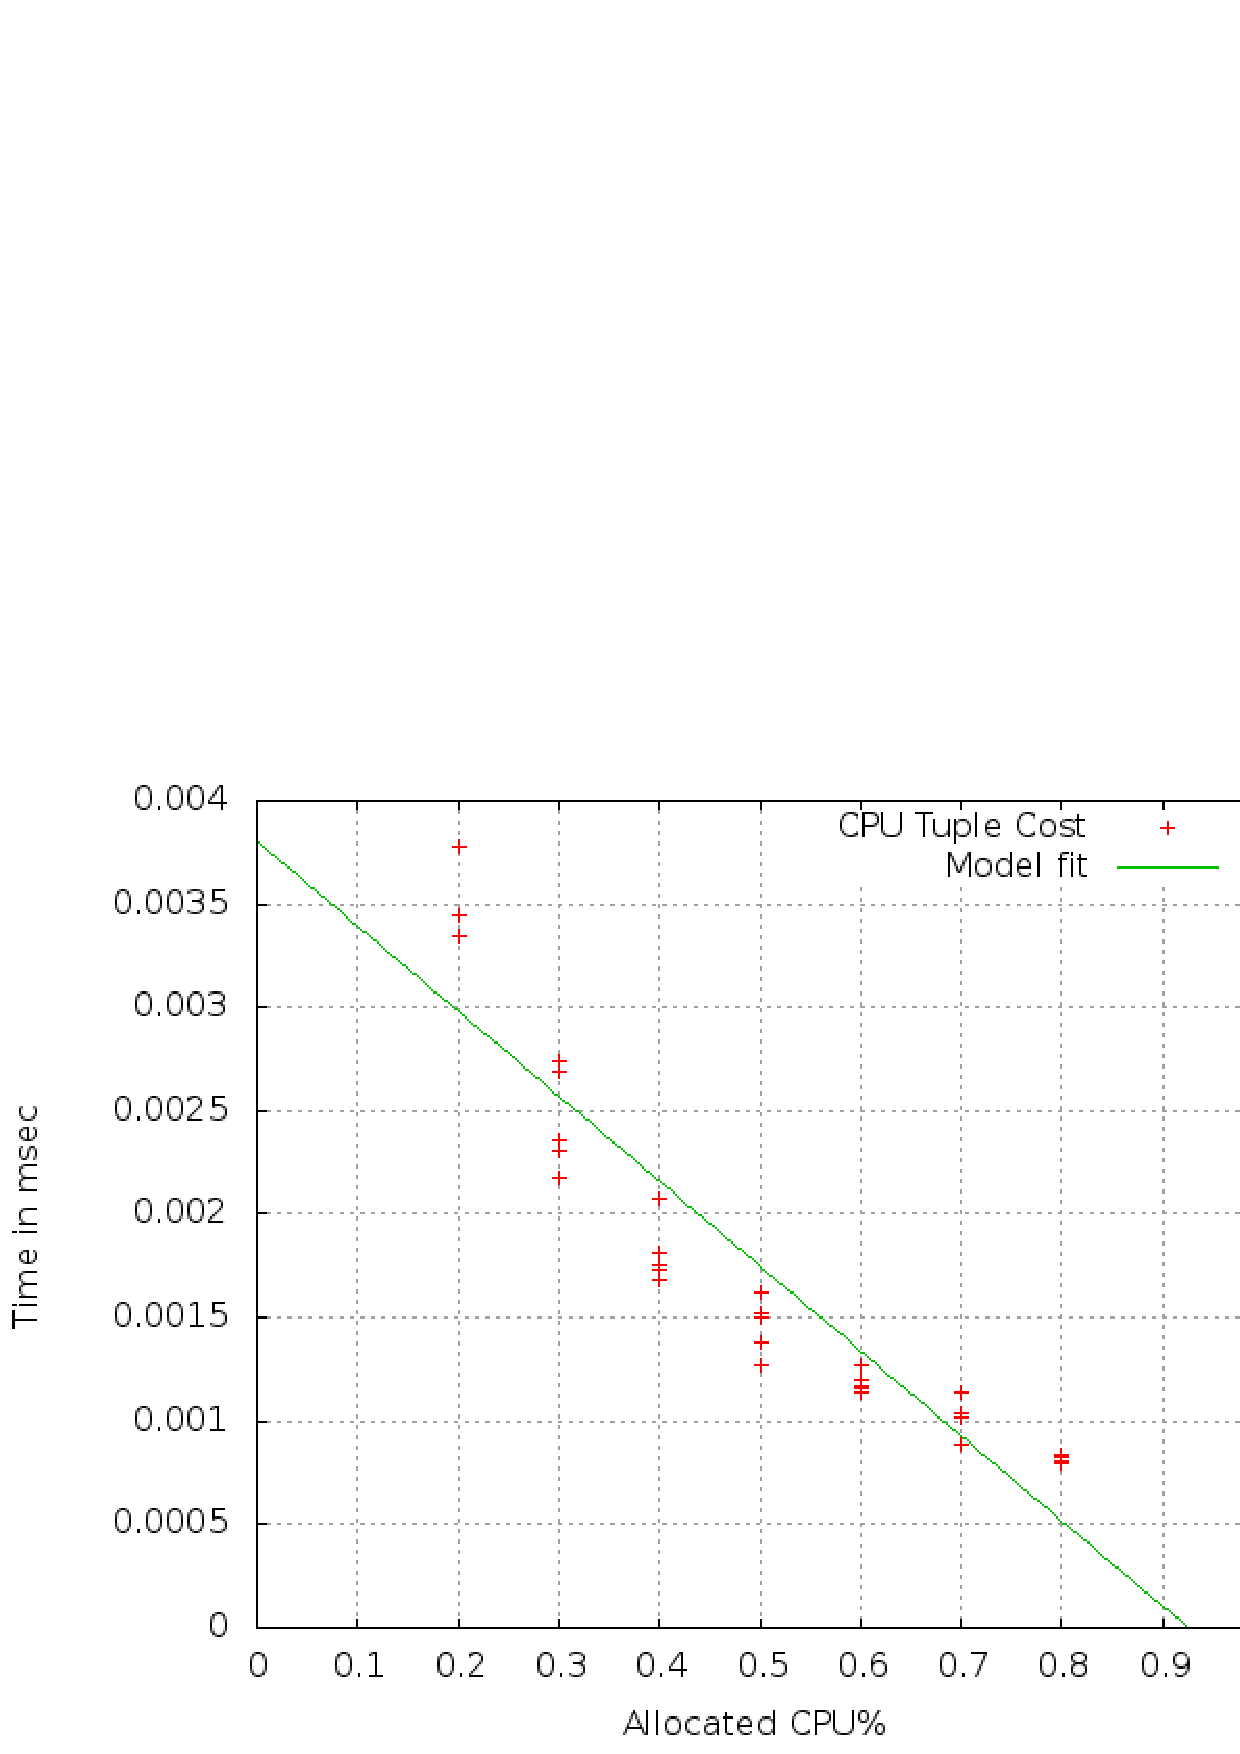
\includegraphics[width=0.8\textwidth]{cpu-tuple-cost.png}
 \caption{$cpu\_tuple\_cost$ calibration}
 \label{fig:cputp}
 \end{figure} 
 
 The calibration of the parameter \textbf{cpu\_index\_tuple} was performed according to chapter ~\ref{chap:implementation}. The results were obtained through the execution of the query presented in subsection ~\ref{app:cal2}. They are shown in figure ~\ref{fig:cpuip}. The errors found for linear parameters $m$ and $b$ are approximately $8.6\%$ and $5.1\%$ , respectively.

 \begin{figure}[ht]
 \centering
 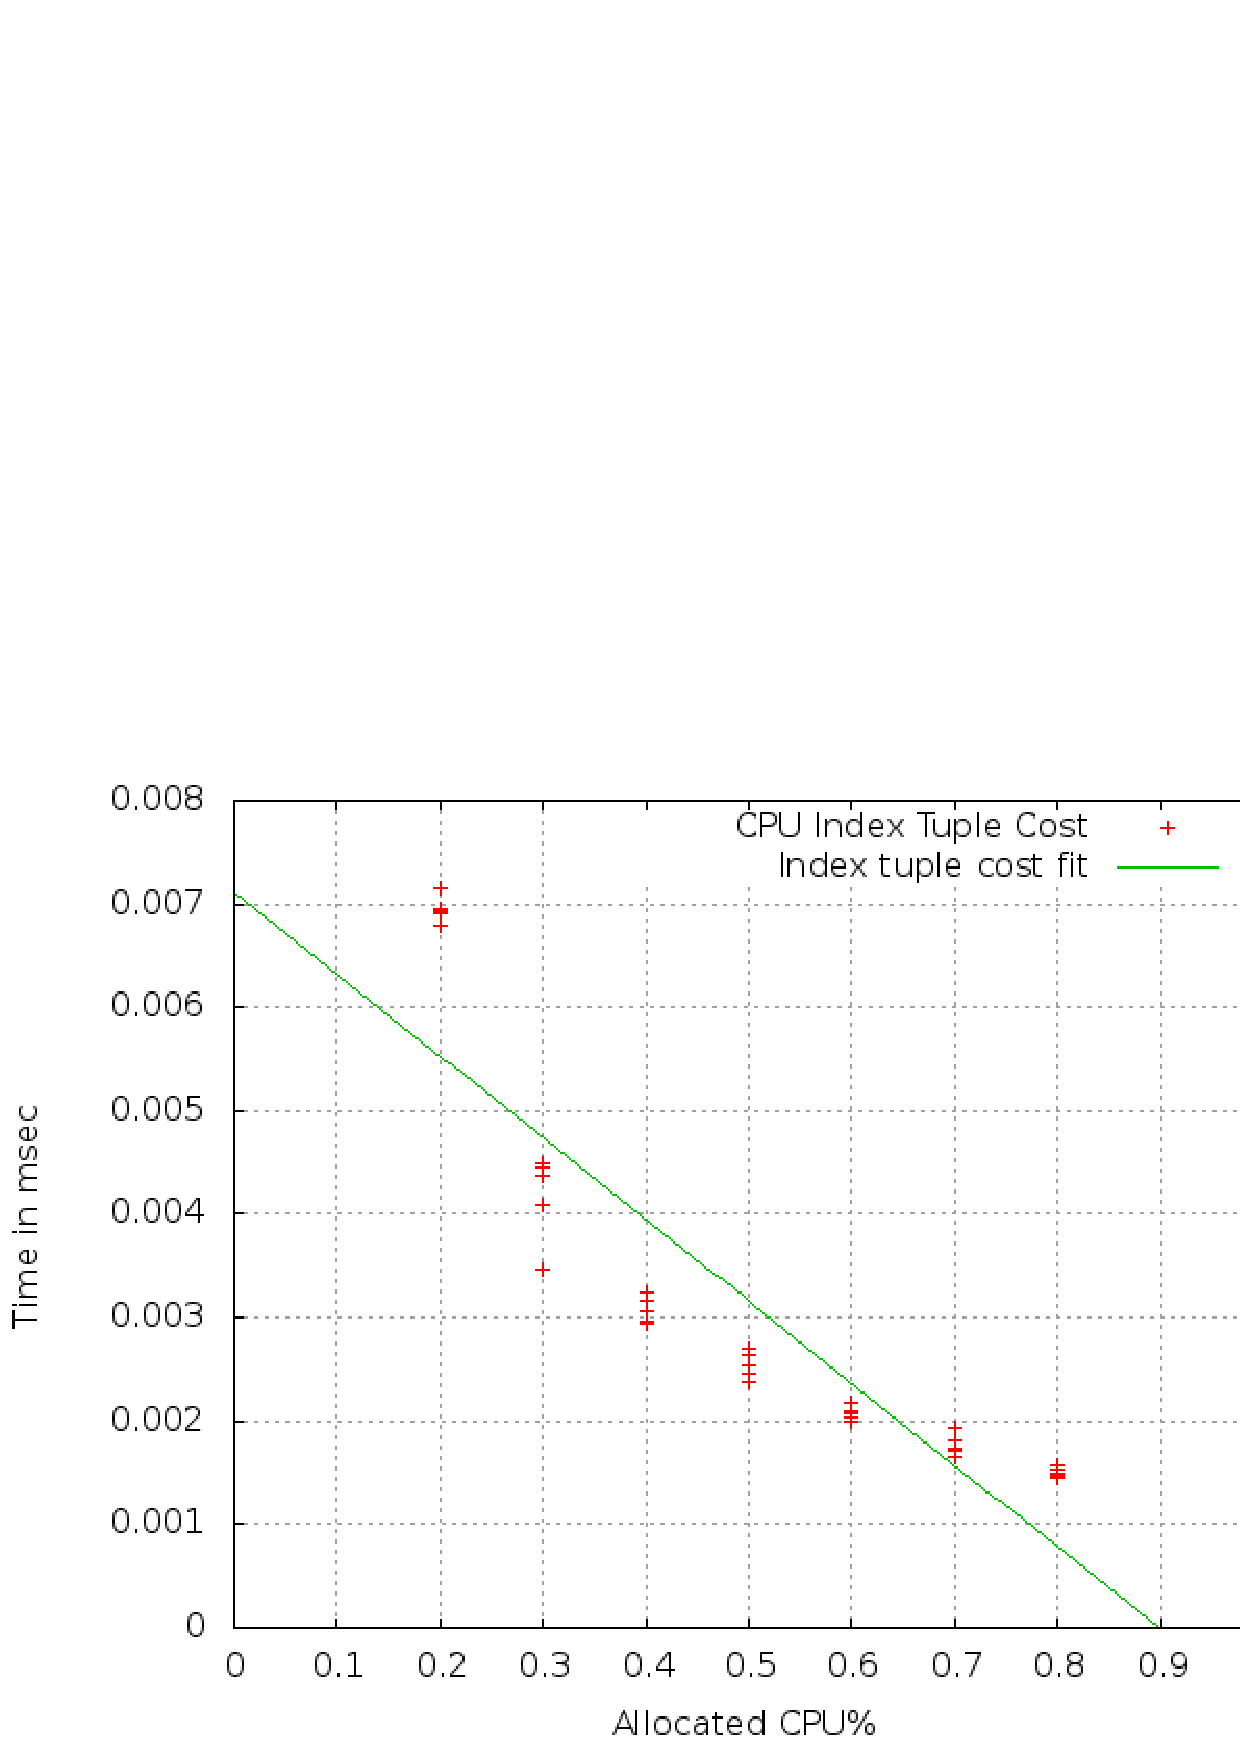
\includegraphics[width=0.8\textwidth]{cpu-index-tuple-cost.png}
 \caption{$cpu\_index\_tuple\_cost$ calibration}
 \label{fig:cpuip}
 \end{figure} 
 
 \section{Advisor}
 
 Once the descriptive parameters are calibrated, it is possible to test the advisor. The tests were performed using TPC-H databases with scale factor 0.6. When loaded into PostgreSQL with their indexes, the size of these databases is $4339 MB$. In order to minimize I/O effects, the databases are also loaded  in a RAM based file system, even though they will not fit entirely in the available RAM. Each database runs in a VM with $1.8 GB$ of RAM.  Each virtual machine is assigned one virtual CPU, during the tests they are pinned to the same core. This magnifies the problem of CPU competition among VM guests, especially in our case, where the workloads are sequentially run.
 
 To measure the performance of our advisor, we compare the costs of running the workloads under the recommended resource allocation to the default allocation. The default consists in simply allocating $1/N$ of the available CPU to the $N$ virtual machines. We consider $T_{default}$ and $T_{advisor}$ to be the execution time of the $N$ workloads running under the default resource allocation and the recommended one, respectively. The performance metric, defined in \cite{Soror:2008:AVM:1376616.1376711}, is the following:
 \[
  \frac{T_{default}-T_{advisor}}{T_{default}}
 \]
.

In our first experiment, we show that the advisor can respond to different workload needs. Two TPC-H queries are used for this experiment, Q18 and Q21. In \cite{Soror:2008:AVM:1376616.1376711}, Q18 is described as one of the most CPU intensive queries. On the other hand, Q21 is one of the least CPU intensive queries, but it is much more I/O intensive than Q18. Based on these queries, two workload units are created. The first is the CPU-intensive workload unit, called C, which consists in instances of Q18. The second is the CPU non-intensive workload unit, called I, built with Q21 instances. Both of these units are scaled to have approximately the same execution time.

Based on these workload units, we create two workloads that are run by two different virtual machines. They are shown below:
\begin{eqnarray*}
 W_{1} &=& 5*C + 5*I \\
 W_{2} &=& k*C + (10-k)*I, 0 \leq k \leq 10. \\
\end{eqnarray*}
As $k$ increases, $W_{2}$ becomes more CPU intensive, while $W_{1}$ remains the same. The correct decision to be taken by our advisor as $k$ increases is to give $W_{2}$ more CPU. The results obtained are shown in figure ~\ref{fig:intensity}. For small $k$, the advisor is able to detect that $W_{2}$ is less CPU intensive, and most of the CPU allocation is given to $W_{1}$. The overall performance is improved  over the default allocation. As $k$ approaches $5$, the workloads become more alike. In this case, improvement is not possible. When $k$ is above $6$, new improvement  opportunities can be found by allocating more CPU to $W_{2}$. However the improvement is not at the same level as before, because both workloads are significantly CPU intensive. This means that the additional CPU allocation, given to $W_{2}$, causes a major performance decrease in $W_{1}$.

\begin{figure}[ht]
 \centering
 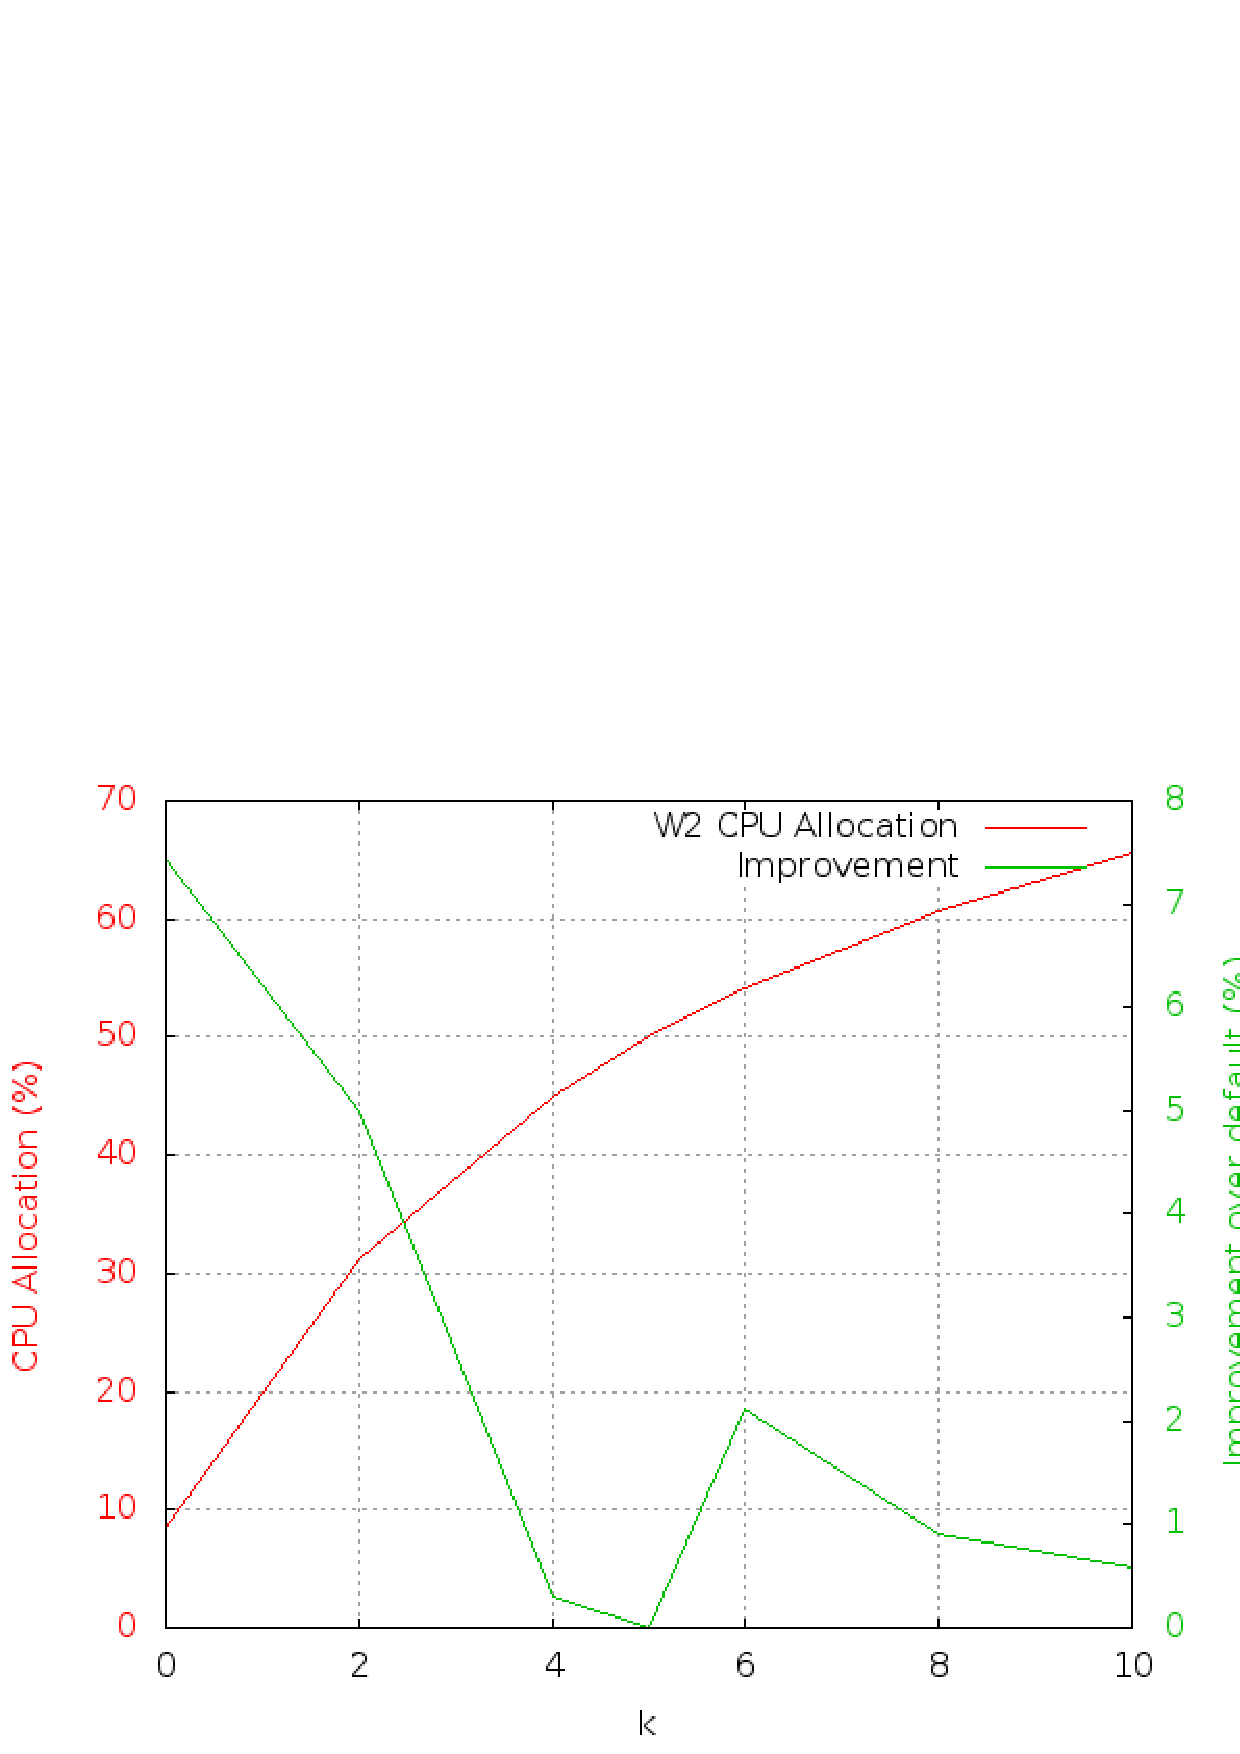
\includegraphics[width=0.8\textwidth]{improvement.png}
 \caption{Varying CPU intensity}
 \label{fig:intensity}
\end{figure} 

The first experiment was also performed in \cite{Soror:2008:AVM:1376616.1376711} for two DBMSes, PostgreSQL 8.1.3 and DB2\footnote{http://www-01.ibm.com/software/data/db2/} V9.  The results obtained for PostgreSQL are significantly worse than those achieved in our implementation, specially for small $k$. They are shown in figure ~\ref{fig:cpuvar-psql}. The improvement rates found in \cite{Soror:2008:AVM:1376616.1376711} are generally below $2\%$. However, they are not very clear about where the TPC-H databases are loaded ( i.e. what type of file system and hardware was used ) and whether the I/O is proportionated among VMs or not. Furthermore, since they use Xen\footnote{http://www.xen.org/} as their hypervisor, they don't specify what type of virtualization technology they use. Xen supports both paravirtualization and hardware assisted virtualization. The virtualization choice affects the performance obtained during execution, although describing how the performance is affected is out of the scope of this paper.

\begin{figure}[ht]
 \centering
 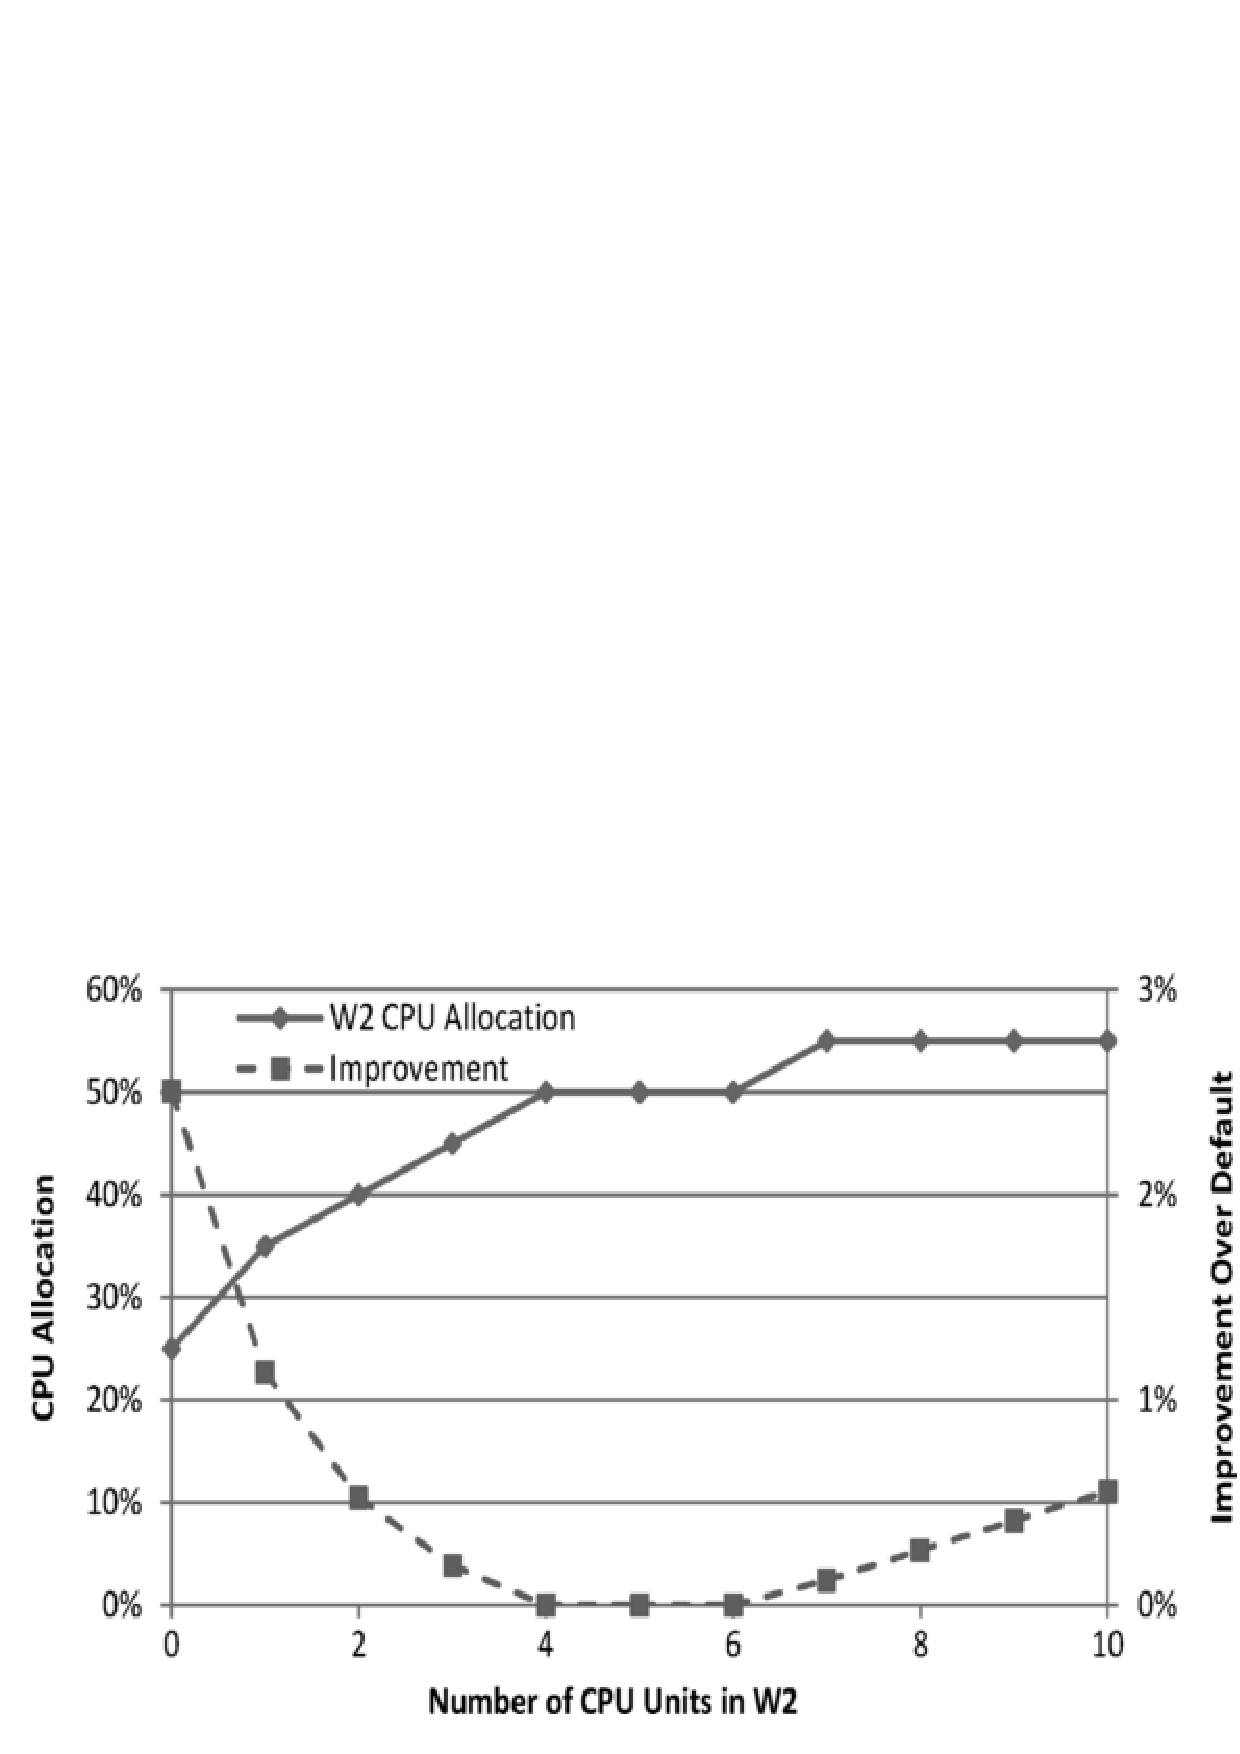
\includegraphics[width=0.8\textwidth]{CPU-var-psql.png}
 \caption{CPU intensity variation for PostgreSQL in \cite{Soror:2008:AVM:1376616.1376711}}
 \label{fig:cpuvar-psql}
\end{figure} 

\subsection{Online Refinement}

The objective of the online refinement is to correct errors in the cost estimator model. However, it also adapts the cost model to small changes in the workload. This means that there are two ways of testing this feature. The first is to run workloads for which the DBMS cost estimator has wrong estimates about. In this case, the errors need to be known beforehand. The second way of testing it is by analyzing how the advisor behaves for small changes in the workload. Using this second approach, we adapt the workloads presented in the first experiment in a second test. Although the online refinement was not disabled in the previous experiment, the workload did not change its needs along the execution. In this second experiment, we test the online refinement feature by modifying the workload along the execution. As $k$ increases, our advisor will try to adapt the model to these changes.

In this test $W_{1}$ and $W_{2}$ are defined as follows:
\begin{eqnarray*}
 W_{1} &=& 3*C + 2*I \\
 W_{2} &=& k*C + (5-k)*I, 0 \leq k \leq 2. \\
\end{eqnarray*}

We vary $k$ from $0$ to $2$ for $W_{2}$, while $W_{1}$ remains unchanged. Instead of comparing the results of the online refinement exclusively to the default allocation, we also compare it to the case in which only the initial configuration search is enabled. This way it is possible to analyze how disabling the online refinement and maintaining static decisions about the workloads may affect the overall performance. The results are shown in figure ~\ref{fig:online-ref-pf}. There it can be seen that without the online refinement, the performance is actually decreased. This happens because $W_{2}$ is treated as a CPU non-intensive workload all the time, thus its CPU needs are underestimated.
\begin{figure}[ht]
 \centering
 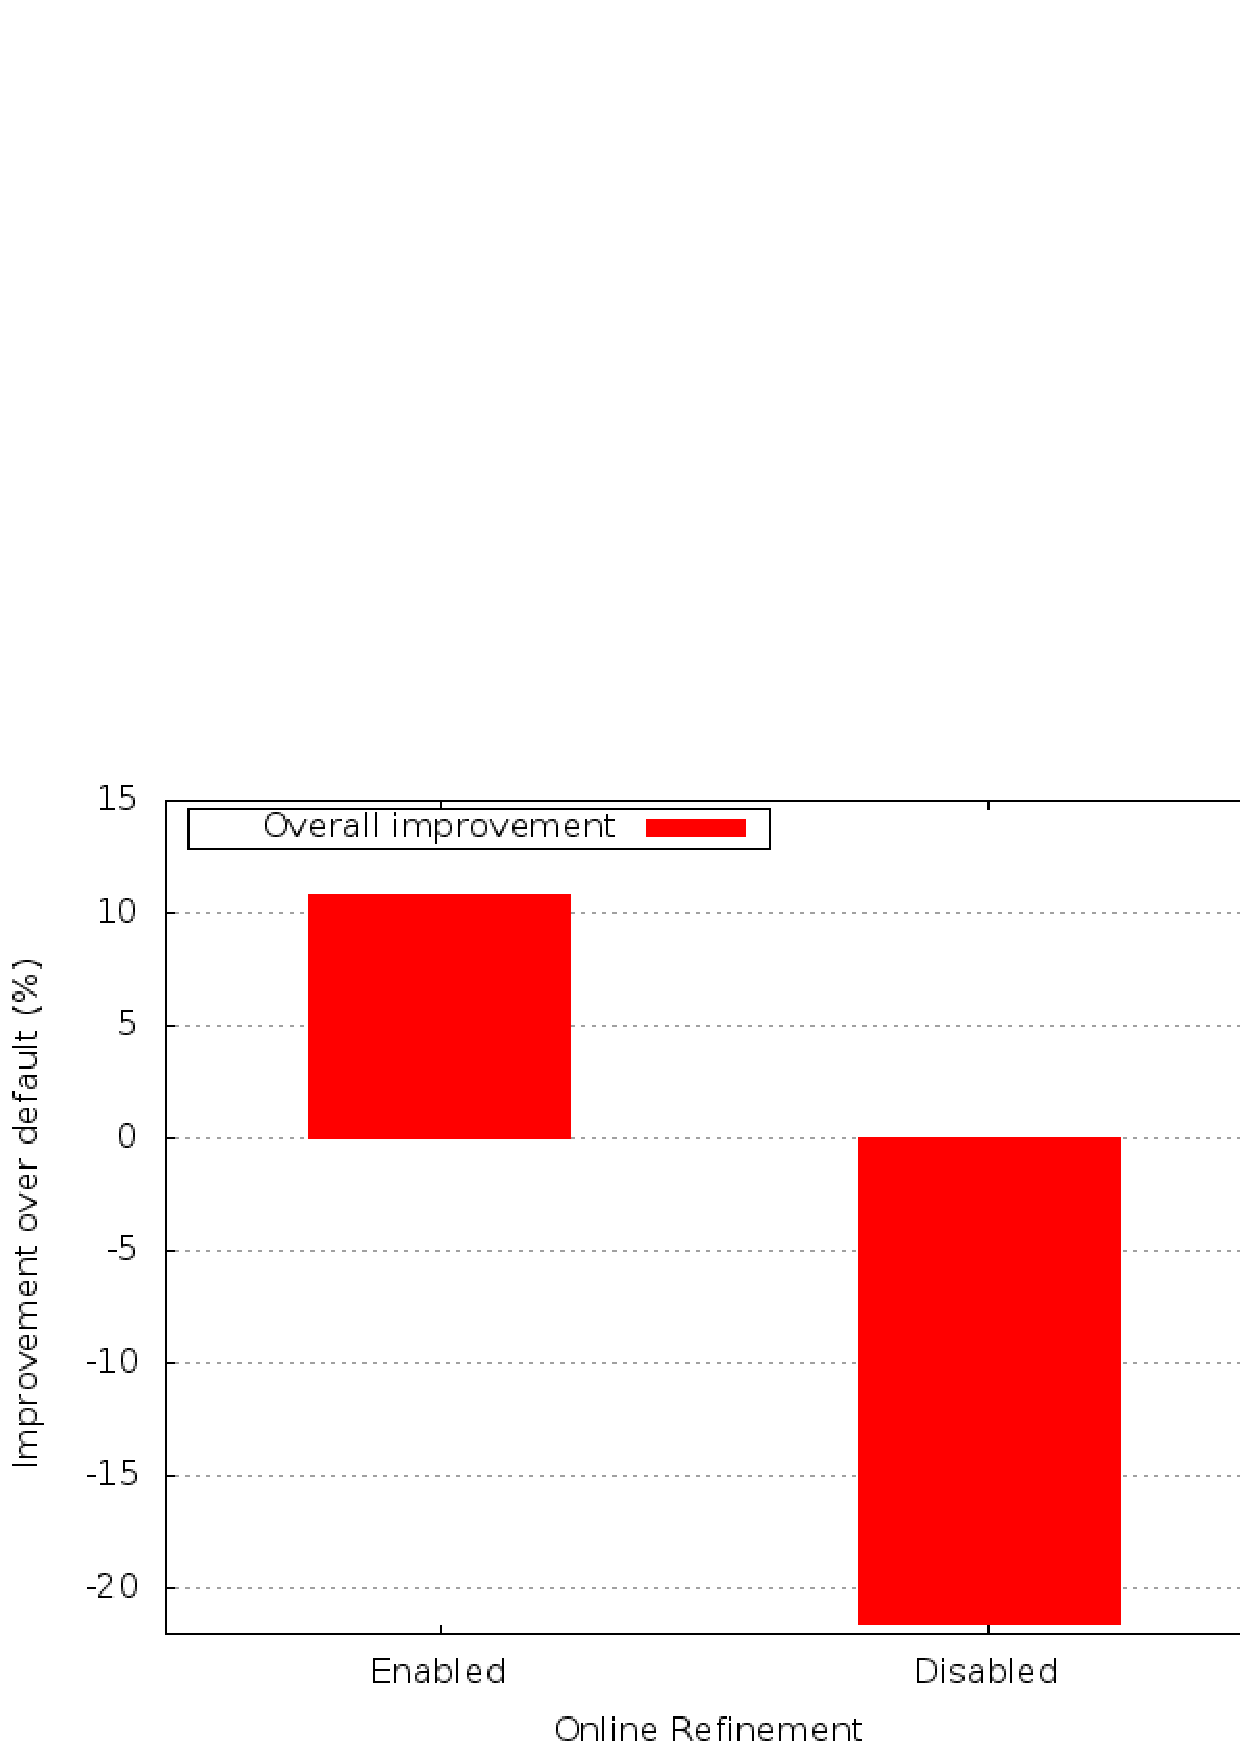
\includegraphics[width=0.8\textwidth]{online-ref.png}
 \caption{Online refinement efficiency}
 \label{fig:online-ref-pf}
\end{figure} 

\subsection{Dynamic Configuration Management}

In OpenRC, this module is responsible for detecting major changes in the workload. In order to test it, it is necessary to cause abrupt changes in the workload needs. This way we are able to see how quickly the restart of the cost model can adjust our estimates. In this test, we compare two TPC-H workloads, called $W_{3}$ and $W_{4}$. Each one of them runs in separate virtual machines. Initially, $W_{3}$ more CPU intensive than $W_{4}$. At some point in execution, these workloads have their characteristics swapped ( i.e. $W_{4}$ becomes more CPU intensive than $W_{3}$ )

This experiment is run twice. At the first time, the dynamic configuration management is disabled. This means that we rely only on the online refinement for correcting the cost model. For the second run, we enable the detection for major workload changes. Our objective is to find out how faster we are able to achieve an optimal allocation by restarting the cost model from scratch.

The advisor is set up to monitor the workloads for changes at each $960$ seconds, and it will consider changes above $20\%$ in CPU needs as major changes. The workloads are split in several units. In figure ~\ref{fig:wkchanges}, we show the CPU allocation along the workload execution organized in periods. Each period defines a moment in which the configuration search was called. The class \textbf{DynamicConfigurationManagement} checks for workload changes just before the fourth period, while the actual swap in the workload needs starts happening after the third period. Once the workloads stabilize, the workload with high CPU needs should receive approximately $70\%$  of the available CPU. Here we show that by restarting the cost model, we can converge to the optimal value faster. At the fifth step of this experiment, $W_{3}$  was still considered less CPU intensive than $W_{4}$. This would incur in a much bigger problem for workloads that change frequently.

\begin{figure}[ht]
 \centering
 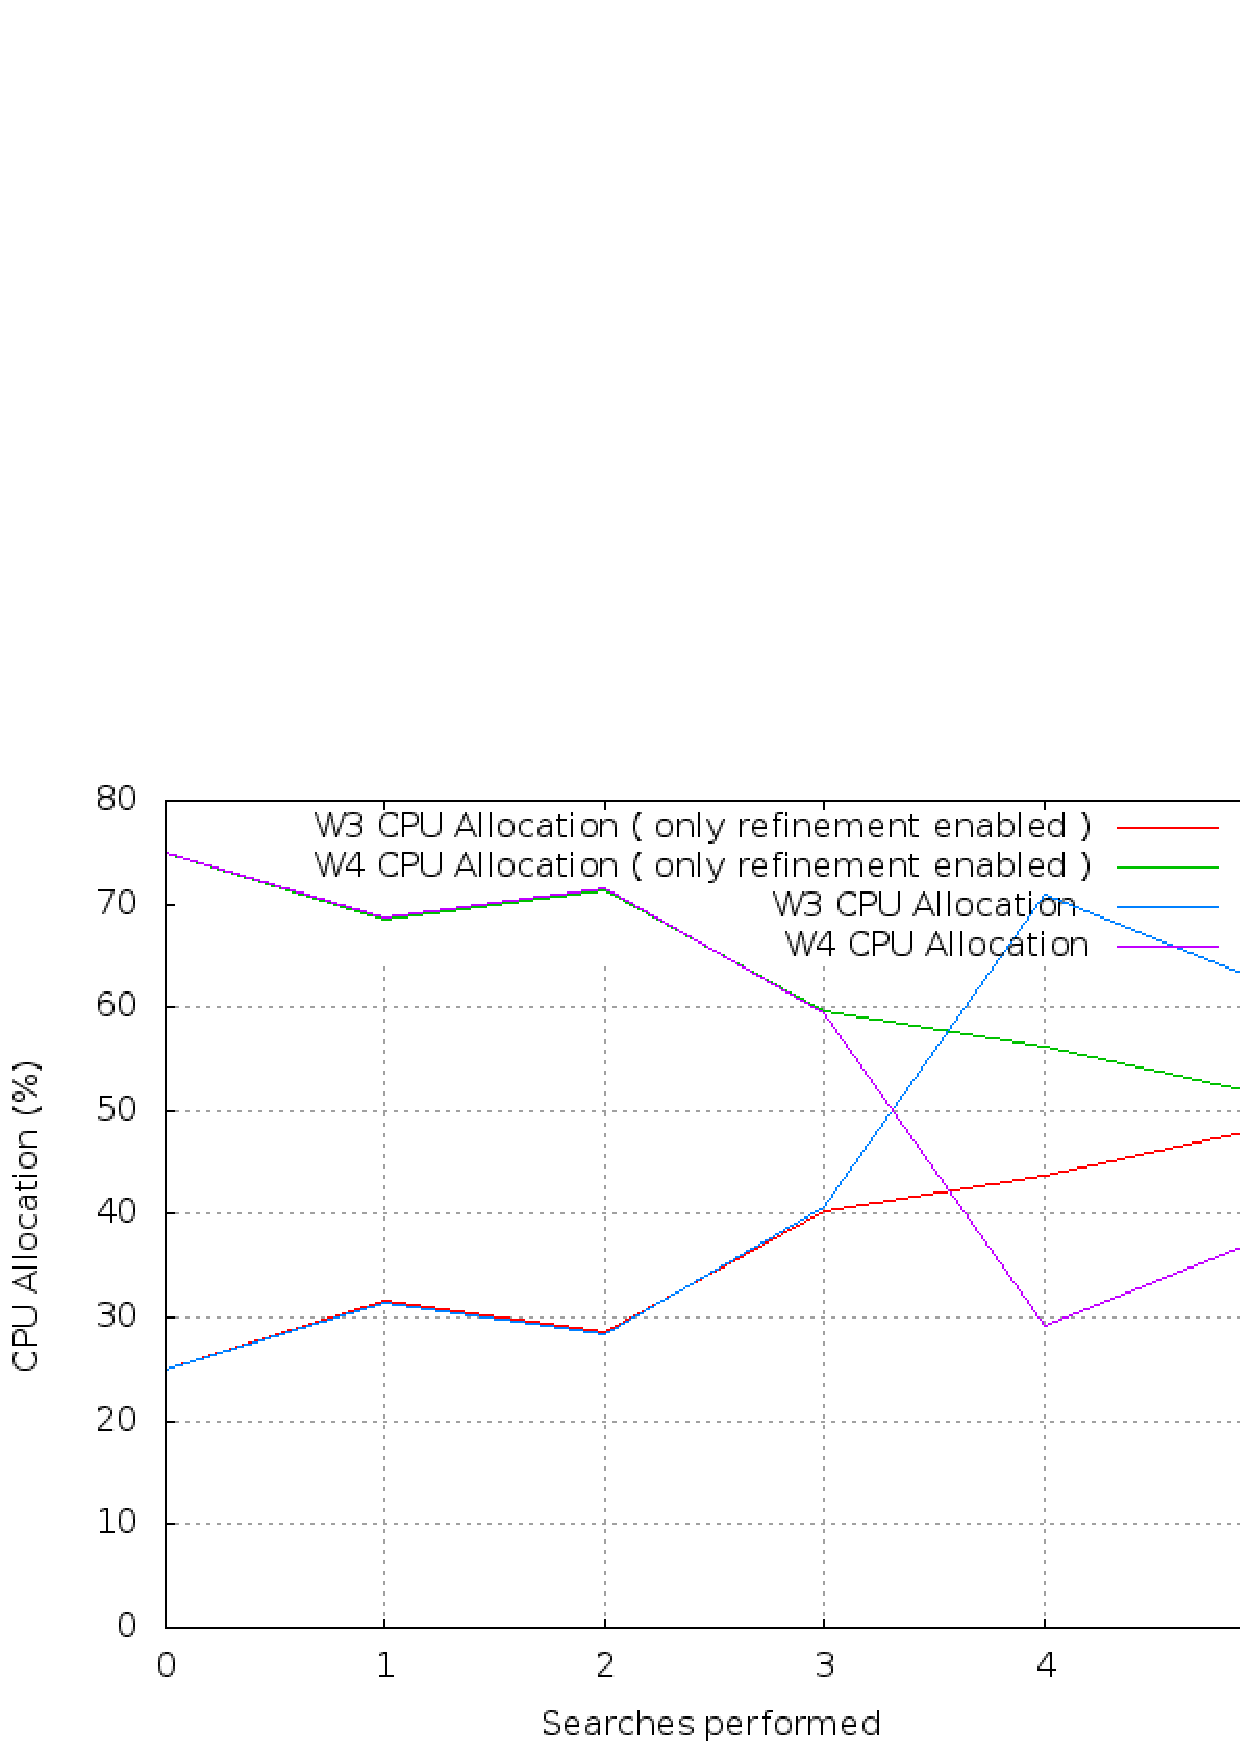
\includegraphics[width=0.8\textwidth]{dyn-change.png}
 \caption{Dynamic workload change detection}
 \label{fig:wkchanges}
\end{figure} 



\chapter{\textbf{Final considerations}}

Even though OpenNebula's capabilities of scheduling enables a way of distribution of resources, this is not enough for consolidating resources. Its goal is not to analyze the application workload inside a VM. That's why the resources need to be required in a static way, in which it's not possible to reallocate resources.

The virtualization design advisor is a way of distributing these resources by considering the database workload. Although it generates overhead, it provides a way of dealing with both over- and under- utilization of resources. 


For a future work, the cloud infrastructure should be more exploited. Through live migration of VMs, a technology already supported by most hypervisors and OpenNebula, it's possible to transfer VMs from one host to another. This could be useful in cases which avoiding over-utilization of resources is not possible ( e.g. Too many VMs with high CPU needs ). This paper was limited to optimize the hosts internally.
%\input{capitulo6.tex}
\chapter{Appendices}

\section{Greedy search algorithm}

\label{sec:greedy}

\begin{algorithm}[H]
 \begin{algorithmic}
    \FOR{$i = 1 \to N$} 
	\STATE $R_{i} \gets [\frac{1}{N},..,\frac{1}{N}]$
    \ENDFOR

   \STATE $done \gets \FALSE$
   \REPEAT
	\STATE $MaxDiff \gets 0$
	\FOR{$j = 1 \to M$} 
	    \STATE $MaxGain_{j} \gets 0$
	    \STATE $MaxLoss_{j} \gets \infty$
	    \FOR{$i = 1 \to N$}
		 \STATE $C' \gets G_{i} * Cost(W_{i},[r_{i1},  r_{ij} + \delta, r_{iM}])$ \COMMENT{Maximize gain}
		 \IF{ $C_{i} - C' > MaxGain_{j}$}
		     \STATE $MaxGain_{j} \gets C_{i} - C'$
		     \STATE $i_{gain} \gets i$
		 \ENDIF
		 \STATE $C' \gets G_{i} * Cost(W_{i},[r_{i1},  r_{ij} - \delta, r_{iM}])$ \COMMENT{Minimize loss}
		 \IF{ $( C' - C_{i} < MaxLoss_{j}) \wedge ( C' satisfies L_{i})$}
		     \STATE $MaxLoss_{j} \gets C' - C_{i}$
		     \STATE $i_{loss} \gets i$
		 \ENDIF
	    \ENDFOR
	    \STATE \COMMENT{Maximum benefit from adjusting this resource}
	    \IF{ $(i_{gain} \ne i_{lose}) \wedge ( MaxGain_{j} - MinLoss_{j} > MaxDiff)$ }
		\STATE $MaxDiff \gets MaxGain_{j} - MinLoss_{j}$
		\STATE $i_{maxgain} \gets i_{gain}$
		\STATE $i_{maxloss} \gets i_{loss}$
		\STATE $j_{max} \gets j$
	    \ENDIF
	\ENDFOR
	\IF{$MaxDiff > 0$}
	    \STATE $r_{i_{maxgain}j_{max}} \gets r_{i_{gain}j_{max}} + \delta $
	    \STATE $r_{i_{maxloss}j_{max}} \gets r_{i_{loss}j_{max}} - \delta $
	\ELSE
	    \STATE $done \gets \TRUE$
	\ENDIF
   \UNTIL{done}

 \end{algorithmic}
  \caption{Greedy search algorithm}
  %\label{alg:greedy}
\end{algorithm}


\section{Calibration queries}

\subsection{cpu\_tuple\_cost and cpu\_operator\_cost}
\label{app:cal1}
\lstinputlisting{./queries/aggregate-seq-scan.sql}

\subsection{cpu\_index\_tuple\_cost}
\label{app:cal2}
\lstinputlisting{./queries/index-scan.sql}
     % se houver anexo




\nocite{*}
\bibliographystyle{plain}
\bibliography{tg}
% utilize macros (3 primeiras letras do mes em ingles, minusculas) no seu
% .bib para atribuir o nome do mes em portugues nas referencia,
% se o style for brazil, outros estilos tambem aceitam estas macros
% Ex:
%
% @InProceedings{teste,
%   author =       {Luciano}
%   year =         {2000}
%   month =        {}#sep;
% }
%
\addcontentsline{toc}{chapter}{\MakeUppercase{References}}


\singlespacing
\makecapadissertacao

\end{document}
